\chapter{线性空间、映射与坐标}
\label{chap:linear-representation}
\label{chap:linear-algebra-and-matrix-analysis}
\label{chap:linear-algebra}

第~\ref{chap:linear-operations}章把数据记成数组，并规定了数组之间的运算，但始终没有追问数组记录的是什么。同一区间上的仿射函数$f_{a,b}(t)=a+bt$是一个完整的函数，两个这样的函数相加、缩放后仍是仿射函数。只有选定$1$与$t$这两个“方向”以后，它才被记录成一列数$(a,b)^{\top}$；换一组方向，记录的数就跟着改变，函数本身却不变。设计矩阵$\bm X_\varepsilon$（式~\eqref{eq:linear-algebra-nearly-collinear-design}）也是如此：它既是一张$3\times2$的数表，也记录了一个把两个系数送到三个拟合值的作用。要在不同记录之间换算而不被记录方式误导，必须把对象与记录对象的数分开。

本章围绕这一区分讨论三个问题：哪些对象能够作线性组合，怎样选取一组足以唯一表示对象的基，以及保持线性组合的作用会丢失或保留什么信息。线性泛函则从另一个方向观察同一空间：它把向量线性地读成一个标量。

我们先建立线性空间和子空间，再用基、维数与坐标描述其中的元素。随后把线性作用记为矩阵，借核与像区分消失的输入和可达到的输出；最后讨论线性泛函及对偶映射。本章主要在实线性空间中展开，涉及复数时会说明标量取值的变化。长度、收敛和正交需要额外结构，由下一章建立。

% 第5章第1节：线性空间与子空间（向量空间；子空间及其包含、交、和、直和与商空间）。

\section{线性空间与子空间}
\label{sec:ls-vector-spaces}
\label{sec:linear-algebra-vector-spaces-coordinates}

第~\ref{chap:linear-operations}章的向量与矩阵、本章开头的仿射函数都可以相加和缩放。要用一组方向去记录这些对象，先得说清楚记录在什么范围里进行。本节回答两个问题。第一，哪些对象可以放在一起作线性组合，并且结果仍是同类对象；这由向量空间的定义回答。

第二，在这样的空间内部，哪些部分自己也能作线性组合而不越界，几个这样的部分怎样比较与合并，有意忽略某个部分里的差别以后又剩下什么；这由子空间及其运算回答。怎样在一个空间里选出一组“尺子”、空间有多大，是下一节的问题。

\subsection{线性空间的定义与示例}
\label{sec:ls-space-axioms}

第~\ref{sec:ls-vector-operation-rules}节验证过，同形数组的加法与数乘满足八条运算规则。平面上的位移可以首尾相接，有限信号可以按幅度放大，多项式可以逐点相加，它们同样满足这些规则：两个对象可以相加，一个对象可以乘以实数，结果仍是同类对象，运算按熟悉的方式交换、结合与分配。后面关于“能否分解、方程有无解、维数是多少”的结论只用到这些规则，与对象具体是数组、位移、信号还是多项式无关。因此把满足这些规则的集合统称为线性空间，其中的元素统称为向量；“向量”从此指可以作线性组合的对象，不再要求它是一列数。

\begin{definition}[实线性空间]
\label{def:ls-real-vector-space}
设$V$是一个集合，给定加法（任意$\bm u,\bm v\in V$对应$\bm u+\bm v\in V$）与实数数乘（任意$a\in\mathbb R$、$\bm u\in V$对应$a\bm u\in V$）。若对任意$\bm u,\bm v,\bm w\in V$和$a,b\in\mathbb R$，下面八条规则成立，就称$V$为\term{向量空间}（也称线性空间，vector space）：
\begin{enumerate}
 \item 加法交换律：$\bm u+\bm v=\bm v+\bm u$。
 \item 加法结合律：$(\bm u+\bm v)+\bm w=\bm u+(\bm v+\bm w)$。
 \item 零元：存在$\bm0\in V$，使$\bm u+\bm0=\bm u$对每个$\bm u$成立。
 \item 加法逆元：每个$\bm u$都有$-\bm u\in V$，使$\bm u+(-\bm u)=\bm0$。
 \item 数乘结合律：$a(b\bm u)=(ab)\bm u$。
 \item 数乘对数的分配律：$(a+b)\bm u=a\bm u+b\bm u$。
 \item 数乘对向量的分配律：$a(\bm u+\bm v)=a\bm u+a\bm v$。
 \item 单位数乘：$1\bm u=\bm u$。
\end{enumerate}
\end{definition}
定义包含两层要求。第一层是\emph{封闭}：加法和数乘的结果必须留在$V$中，否则运算根本无法在$V$内进行。第二层是\emph{规则}：前四条说加法和数的加法一样可以交换、结合，有零元和相反元；后四条说数乘与加法按熟悉的方式配合。

有了这些规则，有限次线性运算无论怎样加括号、怎样展开，都给出同一结果。于是对任意$\bm v_1,\ldots,\bm v_k\in V$与实数$a_1,\ldots,a_k$，加权和$\sum_{j=1}^ka_j\bm v_j$都有确定的意义，仍称为这组向量的线性组合，与第~\ref{sec:ls-vector-operations}节对数组的定义一致。

常见的具体空间都满足定义。$\mathbb R^d$与全部$m\times d$实矩阵在逐项运算下是线性空间，第~\ref{sec:ls-vector-operation-rules}节已逐条验证。次数不超过$k$的实多项式组成的集合$P_k=\{a_0+a_1t+\cdots+a_kt^k\}$在逐点相加与数乘下也是线性空间：两个次数不超过$k$的多项式相加、乘以实数以后，次数仍不超过$k$，八条规则则逐点继承实数的运算规则。本章开头的仿射函数族正是$P_1$。

标量也可以取自复数域。复线性空间的加法和数乘仍满足同样的八条规则，但数乘允许任意复数。对同一个集合，允许哪些标量会改变线性结构：复数集合$\mathbb C$作为复线性空间时，每个元素都由$1$的复数倍得到；把数乘限制为实数时，需要$1$与$\mathrm i$两个方向才能表示$a+b\mathrm i$。复数域上的基与线性映射按相同的方式定义，不过涉及内积时必须处理共轭，本章其余推导先在实数域中进行。

并非每个由向量组成的集合都是线性空间。下面两个$\mathbb R^d$的子集沿用$\mathbb R^d$的运算，却分别破坏了加法封闭与数乘封闭。
\begin{example}[反例：仿射约束集与非负向量集]
\label{ex:ls-non-vector-space-sets}
给定：$\mathbb R^d$的两个子集
\[
 \begin{gathered}
S_1=\{\bm x\in\mathbb R^d:x_1=1\}\\
S_2=\{\bm x\in\mathbb R^d:x_j\geq0,\ j=1,\ldots,d\},
 \end{gathered}
\]
运算沿用$\mathbb R^d$的逐项加法与数乘。

验证：任取$\bm x,\bm y\in S_1$，和的第一坐标为$x_1+y_1=2\neq1$，所以$\bm x+\bm y\notin S_1$；零向量的第一坐标为$0$，所以$S_1$也不含零向量。对$S_2$，两个非负向量之和仍非负，加法封闭；但$\bm e_1\in S_2$，而$(-1)\bm e_1$的第一坐标为$-1$，所以$(-1)\bm e_1\notin S_2$。

结论：$S_1$对加法不封闭，$S_2$对数乘不封闭，二者都不是线性空间。
\end{example}
两个反例说明，判断一个集合是不是线性空间，要逐项检查运算是否封闭、规则是否成立，不能只看集合的形状。

\subsection{子空间、和与直和}
\label{sec:ls-subspaces}
\label{sec:linear-algebra-relations}
\label{sec:linear-algebra-subspace-relations}
\label{sec:ls-subspace-definition}

线性空间$V$中常有一部分元素自己就构成线性空间，例如平面里过原点的一条直线、齐次方程组的全部解。后面的许多问题都落在这样的部分上：一组方向能到达的对象、一个作用消去的输入、方程的解，都不是整个空间。怎样判断$V$的一部分仍是线性空间？

\paragraph{子空间的判定}
设$U$是$V$的非空子集。若$U$对线性组合封闭，即对任意$\bm u,\bm v\in U$和$a,b\in\mathbb R$都有$a\bm u+b\bm v\in U$，就称$U$为$V$的\term{线性子空间}（linear subspace），简称子空间。

这时$U$用$V$的加法与数乘也构成线性空间：取$a=b=1$与$b=0$，分别得到加法与数乘封闭；取$a=b=0$得$\bm0\in U$，取$a=-1,b=0$得$-\bm u\in U$；其余规则对$V$的全部元素成立，自然也对$U$的元素成立。所以判断子空间只需检查这一条封闭条件，不必逐条核对八条规则。

每个空间都有两个平凡子空间：只含零向量的$\{\bm0\}$和$V$本身。下面用判定条件检查三类常见集合。
\begin{example}[过原点的直线、平移的直线与齐次解集]
\label{ex:ls-subspace-checks}
给定：平面中的非零向量$\bm u$，不在直线$\{c\bm u:c\in\mathbb R\}$上的点$\bm p$，以及矩阵$\bm A\in\mathbb R^{m\times d}$。考察
\[
 \begin{gathered}
 L_0=\{c\bm u:c\in\mathbb R\},
 \qquad
 L_1=\{\bm p+c\bm u:c\in\mathbb R\},\\
 N=\{\bm x\in\mathbb R^d:\bm A\bm x=\bm0\}.
 \end{gathered}
\]

验证：在$L_0$中任取$c_1\bm u$与$c_2\bm u$，有$a(c_1\bm u)+b(c_2\bm u)=(ac_1+bc_2)\bm u\in L_0$。在$N$中任取两个解$\bm x,\bm y$，由式~\eqref{eq:prelim-matrix-linearity}，
\[
 \bm A(a\bm x+b\bm y)=a\bm A\bm x+b\bm A\bm y=\bm0,
\]
所以$a\bm x+b\bm y\in N$。$L_1$不含零向量：若$\bm p+c\bm u=\bm0$，则$\bm p=-c\bm u$落在$L_0$上，与$\bm p$的取法矛盾。

结论：过原点的直线$L_0$与齐次线性方程组的解集合$N$都是子空间；不过原点的直线$L_1$不含零向量，不是子空间。
\end{example}
$L_1$是子空间$L_0$沿$\bm p$平移所得。示例~\ref{ex:ls-non-vector-space-sets}中的非齐次约束集$S_1=\{\bm x:x_1=1\}$也是这样，它是齐次解集$\{\bm x:x_1=0\}$沿$\bm e_1$平移所得的仿射集合，同样不是子空间。

固定同一个空间$V$，它的几个子空间之间可以问四个问题：一个是否装得下另一个，二者有哪些公共方向，合在一起能到达哪里，合并后的分解是否唯一。这四个问题分别由包含、交、和与直和回答。这里比较的都是线性范围，不涉及长度或夹角。

最后再问一个方向相反的问题：若把某个子空间里的差别有意忽略，剩下的对象是否仍构成线性空间？这由商空间回答。

\paragraph{包含}
\phantomsection
\label{sec:ls-subspace-inclusion}
若子空间$U$的每个元素都属于子空间$W$，就记$U\subseteq W$。这时$U$在$W$中对线性组合封闭，因而也是$W$的子空间。包含只比较两个集合的范围；两个子空间的“大小”怎样比较，要等下一节定义维数以后才能回答。

\paragraph{交}
\phantomsection
\label{sec:ls-intersection}
两个子空间$U,W\subseteq V$的交$U\cap W$由同时属于二者的元素组成。它仍是子空间：$\bm x,\bm y\in U\cap W$时，二者既在$U$中也在$W$中，故$a\bm x+b\bm y$同属两边。交也是同时包含在$U$与$W$中的最大子空间，因为任何同时含于两边的子空间，其元素都属于交。在平面中，两条重合的过原点直线的交是整条直线，两条不同的过原点直线的交只有零向量。交为零只说明两个子空间没有公共的非零方向，并不说明二者合起来能到达整个空间：$\mathbb R^3$中两条不同的过原点直线交为零，合起来却只能到达一个平面。

当$U,W$分别由齐次线性方程组描述时，交就是同时满足两组方程的解集合。例如$U=\{\bm x:x_1=0\}$与$W=\{\bm x:x_2=0\}$的交是$\{\bm x:x_1=x_2=0\}$。这样，求交就化为解联立的齐次方程组，具体的消元方法留到第~\ref{chap:linear-equations-and-optimization}章。

\paragraph{和}
\phantomsection
\label{sec:ls-sum}
两个子空间中的向量相加，所能到达的对象组成和空间$U+W=\{\bm u+\bm w:\bm u\in U,\ \bm w\in W\}$。它对线性组合封闭：
\[
 a(\bm u_1+\bm w_1)+b(\bm u_2+\bm w_2)=(a\bm u_1+b\bm u_2)+(a\bm w_1+b\bm w_2),
\]
右端两个括号分别属于$U$与$W$。任何同时包含$U,W$的子空间都必须含有每个$\bm u+\bm w$，所以$U+W$是同时包含二者的最小子空间。

为什么不直接用并集$U\cup W$？因为并集一般对加法不封闭。
\begin{example}[反例：两条坐标轴的并]
\label{ex:ls-union-not-subspace}
给定：$\mathbb R^2$中的两个子空间$U=\{(s,0)^\top:s\in\mathbb R\}$与$W=\{(0,s)^\top:s\in\mathbb R\}$，即两条坐标轴。

验证：$\bm e_1\in U$、$\bm e_2\in W$，二者都属于$U\cup W$；但$\bm e_1+\bm e_2=(1,1)^\top$的两个坐标都不为零，既不在$U$中，也不在$W$中。

结论：$U\cup W$对加法不封闭，不是子空间；包含$U$与$W$的最小子空间是$U+W=\mathbb R^2$。
\end{example}
和空间正是在并集之外补入了$\bm u+\bm w$这类必要的线性组合。

\paragraph{直和与补空间}
\phantomsection
\label{sec:ls-direct-sum}
和空间中的向量能写成$\bm u+\bm w$，但写法未必唯一。在平面上，一条过原点的直线只能到达部分方向；再取一条不平行的过原点直线，平面中的每个向量都能拆成分别落在两条直线上的两部分，而且拆法唯一。怎样把“拆法唯一”写成两个子空间之间的条件？

条件是两个子空间只交于零向量：$U+W$中每个向量的分解$\bm u+\bm w$都唯一，当且仅当$U\cap W=\{\bm0\}$。

先证充分性。若$\bm u_1+\bm w_1=\bm u_2+\bm w_2$，移项得$\bm u_1-\bm u_2=\bm w_2-\bm w_1$；左边在$U$中，右边在$W$中，所以这个向量属于$U\cap W$，只能是零，于是$\bm u_1=\bm u_2$、$\bm w_1=\bm w_2$。

再证必要性。若交中有非零向量$\bm z$，则$\bm z\in U$、$-\bm z\in W$，等式$\bm0=\bm0+\bm0=\bm z+(-\bm z)$给出零向量的两种不同分解，唯一性失败。

满足$U\cap W=\{\bm0\}$时，称和$U+W$为\term{直和}（direct sum），记为$U\oplus W$。唯一分解不要求两个子空间互相垂直：平面中任意两条不平行的过原点直线都构成直和。

若还有$U+W=V$，就写$V=U\oplus W$，这样的$W$称为$U$在$V$中的\term{补空间}（complement）。补空间一般不唯一：在平面中给一条过原点的直线选补空间，任何不平行于它的过原点直线都可以。补空间是否总存在，要用到下一节的基扩充（第~\ref{sec:ls-dimension}节）。指定内积以后的正交补是另一回事，由第~\ref{sec:ls-orthogonality}节介绍，不能把一般补空间自动称为正交补。

\subsection{商空间}
\phantomsection
\label{sec:ls-quotient-spaces}
\label{sec:linear-algebra-equivalence-relations}
前面的运算都在合并子空间；有时却要反过来，把某个子空间里的差别有意忽略。例如只读取仿射函数$f_{a,b}(t)=a+bt$在$t=0$处的值，即截距$a$时，$f_{a,b}$与$f_{a,b'}$没有区别，二者之差$(b-b')t$落在子空间$\{st:s\in\mathbb R\}$中。

前面的非齐次约束$x_1=1$也是如此：它的解集合$\{\bm e_1+\bm n:n_1=0\}$由一个特解加上齐次解子空间$\{\bm n:n_1=0\}$中的全部向量组成，任意两个解之差都落在这个子空间里。两个例子的共同点是：相差某个子空间中的向量，就被视为相同。

把这一共同点写成关系：设$U$是$V$的子空间，规定$\bm x\sim\bm y$当且仅当$\bm x-\bm y\in U$。这是第~\ref{chap:sets-functions-and-proofs}章定义~\ref{def:prelim-equivalence-relation}意义下的等价关系：$\bm x-\bm x=\bm0\in U$给出自反性；$\bm x-\bm y\in U$蕴含$\bm y-\bm x\in U$，给出对称性；$(\bm x-\bm y)+(\bm y-\bm z)=\bm x-\bm z\in U$给出传递性。

$\bm x$的等价类为
\[
 \bm x+U=\{\bm x+\bm n:\bm n\in U\},
\]
即子空间$U$沿$\bm x$平移所得的集合。两个类相等不要求所取的代表元相等，只要求代表元之差落在$U$中。全部等价类把$V$划分成互不重叠的块。图~\ref{fig:ls-quotient-equivalence-classes}在平面上画出这一划分：$U$是$x$轴，每条平行于$x$轴的直线是一个等价类。
\begin{figure}[htbp]
  \centering
  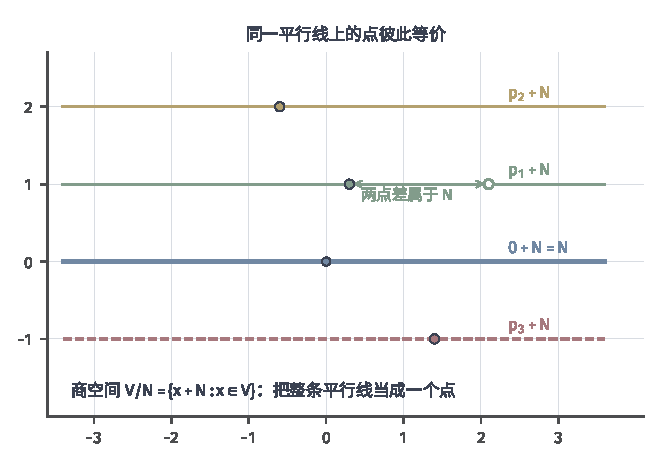
\includegraphics[width=112mm]{figures/00-shared/mathematical-preliminaries-upper/02-linear-spaces/matplotlib/ls-quotient-equivalence-classes/ls-quotient-equivalence-classes.pdf}
  \caption{商空间的等价类。$V=\mathbb R^2$，子空间$U$为$x$轴（蓝线$0+U$）；每条平行直线$p+U=\{(x,p_y)\}$是一个等价类，图中画出$y=1$（绿）、$y=2$（黄）、$y=-1$（红虚线）。绿线上实点$(0.3,1)$与空心点$(2.1,1)$之差$(1.8,0)\in U$，故属同一类；商空间$V/U$把每条平行线当成一个点。}
  \label{fig:ls-quotient-equivalence-classes}
\end{figure}

这些类能否像向量一样相加和缩放？自然的做法是借代表元来算。
\begin{definition}[商空间]
\label{def:linear-algebra-quotient-space}
设$U$是线性空间$V$的子空间。全部等价类$\bm x+U$组成的集合记为$V/U$，规定
\[
 \begin{gathered}
(\bm x+U)+(\bm y+U)=(\bm x+\bm y)+U\\
a(\bm x+U)=a\bm x+U,
 \end{gathered}
\]
称$V/U$为$V$对$U$的\term{商空间}（quotient space）。
\end{definition}
借代表元定义运算，必须先检查结果与代表元的选取无关。换代表元$\bm x'=\bm x+\bm n_1$、$\bm y'=\bm y+\bm n_2$（$\bm n_1,\bm n_2\in U$）时，$\bm x'+\bm y'$与$\bm x+\bm y$只相差$\bm n_1+\bm n_2$，$a\bm x'$与$a\bm x$只相差$a\bm n_1$，二者都属于$U$，所以得到同一个类。

零类是$U$本身，$\bm x+U$的相反类是$-\bm x+U$，其余规则由$V$的运算规则逐条继承，所以$V/U$构成线性空间。在图~\ref{fig:ls-quotient-equivalence-classes}中，两条水平线相加就是把高度相加：商空间只记录高度，被忽略的是沿$x$轴的位置。

回到截距的例子，商空间恰好只保留截距。
\begin{example}[只保留截距的商空间]
\label{ex:ls-quotient-intercept}
给定：$V=P_1=\{a+bt:a,b\in\mathbb R\}$与子空间$U=\{st:s\in\mathbb R\}$。

计算：$f_{a,b}=a+bt$所在的类是
\[
 f_{a,b}+U=\{a+(b+s)t:s\in\mathbb R\}=\{a+rt:r\in\mathbb R\},
\]
它只依赖$a$。两个类$f_{a,b}+U$与$f_{a',b'}+U$相等，当且仅当$f_{a,b}-f_{a',b'}=(a-a')+(b-b')t\in U$，即$a=a'$。按商空间的运算，
\[
 \begin{gathered}
(f_{a,b}+U)+(f_{a',b'}+U)=f_{a+a',\,b+b'}+U\\
c(f_{a,b}+U)=f_{ca,\,cb}+U,
 \end{gathered}
\]
即截距分别相加、缩放。

结论：规则$f_{a,b}+U\mapsto a$是从$P_1/U$到$\mathbb R$的双射，并保持加法与数乘。商空间$P_1/U$只记录截距，被忽略的是斜率。
\end{example}
商空间有多少个独立方向，要等下一节有了维数才能回答（第~\ref{sec:ls-dimension}节）；它与线性映射的联系在第~\ref{sec:ls-kernel-image}节给出。

% 第5章第2节：基、维数与坐标（线性无关与张成、基、维数、坐标与坐标变换）。

\section{基、维数与坐标}
\label{sec:ls-bases-dimension-coordinates}

上一节规定了在什么范围里作线性组合，但还没有回答怎样用有限个数记录一个对象。思路是选定一组方向，把对象写成它们的线性组合，用组合系数代替对象。

这要求依次回答几个问题：一组方向能到达哪些对象；到达同一个对象的系数是否唯一；怎样挑出一组既够用又不重复的方向作为“尺子”；不同的尺子是否总含同样多根，即空间有多大；选定尺子以后，系数怎样代替对象参与计算，换一把尺子系数怎样换算。前一个问题的答案是后一个问题的前提，所以按这个顺序展开。

\subsection{张成与线性无关}

\paragraph{张成}
\phantomsection
\label{sec:ls-span}
在平面上，两个不共线方向的加权组合能取到每一个点；只有一个方向时，无论怎样加权，结果都停在过原点的一条直线上。要描述一组方向“能到达哪里”，先给它们的全部线性组合命名：给定$\bm v_1,\ldots,\bm v_k\in V$，集合
\begin{equation}
 \operatorname{span}\{\bm v_1,\ldots,\bm v_k\}
 =\left\{\sum_{j=1}^k a_j\bm v_j:a_j\in\mathbb R\right\}
 \label{eq:ls-span}
\end{equation}
称为这组向量的\term{张成空间}（span）。

两个线性组合再作线性组合，仍是这组向量的线性组合，所以张成空间对线性组合封闭，是$V$的子空间。

任何包含$\bm v_1,\ldots,\bm v_k$的子空间都必须含有它们的全部线性组合，所以张成空间是包含这组向量的最小子空间。若$\operatorname{span}\{\bm v_1,\ldots,\bm v_k\}=V$，就说这组向量张成$V$，也称它们是$V$的一个生成组。

在$\mathbb R^m$中，把$\bm v_1,\ldots,\bm v_k$排成矩阵$\bm V$的各列，按列读法$\sum_ja_j\bm v_j=\bm V\bm a$，所以张成空间就是$\bm V$乘上全部系数向量所得的输出集合$\{\bm V\bm a:\bm a\in\mathbb R^k\}$，第~\ref{sec:ls-kernel-image}节将把它称为$\bm V$的列空间。如图~\ref{fig:ls-linear-combination-span}所示，两个不共线方向的组合取遍整个平面，单个方向的组合只是一条直线。
\begin{figure*}[htbp]
  \centering
  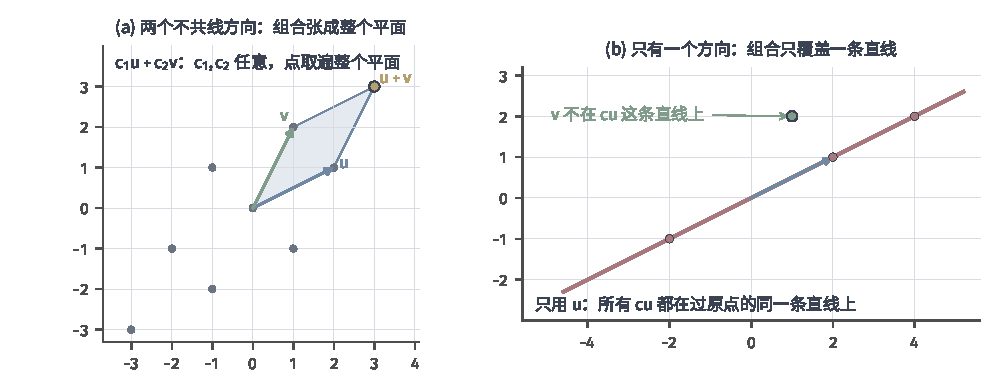
\includegraphics[width=169mm]{figures/00-shared/mathematical-preliminaries-upper/02-linear-spaces/matplotlib/ls-linear-combination-span/ls-linear-combination-span.pdf}
  \caption{两个方向与一个方向的张成范围。左：$\bm u=(2,1)$（蓝箭头）与$\bm v=(1,2)$（绿箭头）的全部加权组合取遍整个平面，浅蓝平行四边形标出$0,\bm u,\bm u+\bm v,\bm v$，灰点为整数系数格点，黄点为$\bm u+\bm v=(3,3)$。右：只有$\bm u$一个方向时，组合$\{c\bm u\}$只是过原点的一条直线（红线），$\bm v$不在其上。两图坐标等比例，为解析教学例。}
  \label{fig:ls-linear-combination-span}
\end{figure*}

\paragraph{线性无关}
\phantomsection
\label{sec:ls-linear-dependence}
张成告诉我们哪些对象能被表示，却没有说明表示方式是否只有一种。若同一个对象可以用两组不同的系数写出，某些方向就是多余的。两组系数相减，就得到零向量的一个系数不全为零的表示，所以判断冗余，只需看零向量能否被非平凡地表示。若
\begin{equation}
 a_1\bm v_1+\cdots+a_k\bm v_k=\bm0
 \label{eq:linear-algebra-independence-relation}
\end{equation}
仅在全部$a_j=0$时成立，就称这组向量\term{线性无关}（linearly independent）；否则称为\term{线性相关}（linearly dependent），即存在不全为零的系数使式\eqref{eq:linear-algebra-independence-relation}成立。线性相关时挑出一个非零系数$a_j$并移项，就能把$\bm v_j$写成其余向量的线性组合，说明这个方向重复了已有方向能到达的范围。在$\mathbb R^m$中，线性无关就是齐次方程$\bm V\bm a=\bm0$只有零解；第~\ref{sec:ls-gram-orthogonality}节还将说明，它等价于Gram矩阵$\bm V^\top\bm V$正定。

贯穿例的两列几乎同向，它们是否线性无关？
\begin{example}[近共线的两列仍线性无关]
\label{ex:ls-nearly-collinear-independence}
给定：式~\eqref{eq:linear-algebra-nearly-collinear-design}中的$\bm c_1=(1,1,1)^\top$、$\bm q=(0,1,-1)^\top$与$\bm c_2=\bm c_1+\varepsilon\bm q$。

验证：先看$\bm c_1$与$\bm q$。$\alpha\bm c_1+\beta\bm q=(\alpha,\ \alpha+\beta,\ \alpha-\beta)^\top$为零时，第一坐标给出$\alpha=0$，第二坐标再给出$\beta=0$，所以$\bm c_1,\bm q$线性无关。再看两列：
\[
 a_1\bm c_1+a_2\bm c_2=(a_1+a_2)\bm c_1+a_2\varepsilon\bm q .
\]
它为零时，由$\bm c_1,\bm q$线性无关得$a_1+a_2=0$与$a_2\varepsilon=0$。

结论：$\varepsilon\neq0$时只能$a_2=0$，进而$a_1=0$，两列线性无关；$\varepsilon=0$时$\bm c_1-\bm c_2=\bm0$，两列线性相关。
\end{example}
所以“两列几乎同向”和线性无关是两回事。线性无关是精确的是非判断，只要$\varepsilon\neq0$就成立；几乎同向描述的是接近退化的程度，要由夹角或Gram矩阵衡量，第~\ref{sec:ls-inner-product-definition}节把这种情形称为近共线。

\paragraph{表示的存在与唯一}
“能表示哪些对象”和“表示是否冗余”是两个独立的问题，分别由张成与线性无关回答。下面的例子在平面上把二者分开。
\begin{example}[足够、不够与冗余的方向组]
\label{ex:ls-redundant-spanning-set}
给定：$\mathbb R^2$中的$\bm v_1=(1,0)^{\top}$、$\bm v_2=(0,1)^{\top}$与$\bm v_3=(1,1)^{\top}$。

计算：第一，$a_1\bm v_1+a_2\bm v_2=(a_1,a_2)^{\top}$，任一目标点$(x,y)^\top$都由唯一的系数$a_1=x$、$a_2=y$取到。第二，只取$\bm v_1$时，组合$a_1\bm v_1=(a_1,0)^\top$只能到达横轴，取不到$\bm v_2$。第三，取$\bm v_1,\bm v_2,\bm v_3$时，能到达的点仍是整个平面，但目标$(1,1)^\top$有两组系数：
\[
 0\bm v_1+0\bm v_2+1\bm v_3=(1,1)^\top=1\bm v_1+1\bm v_2+0\bm v_3 .
\]
两组系数相减，得到零向量的非平凡表示$\bm v_1+\bm v_2-\bm v_3=\bm0$。

结论：$(\bm v_1,\bm v_2)$足够且无冗余；$(\bm v_1)$不够；$(\bm v_1,\bm v_2,\bm v_3)$足够，但表示冗余。
\end{example}
图~\ref{fig:vol1-add-linear-redundant-directions}把第三种情形下的两种表示画到同一个平面上。
\begin{figure}[!htb]
  \centering
  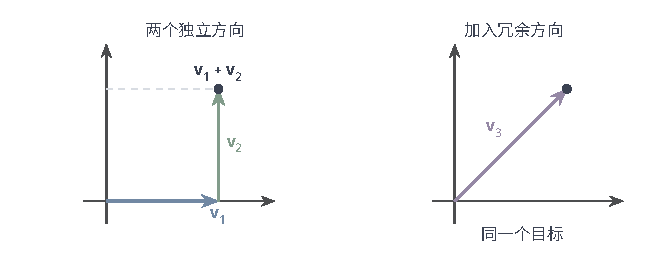
\includegraphics[width=112mm]{figures/00-shared/mathematical-preliminaries-upper/02-linear-spaces/tikz/comprehension-additions/linear-redundant-directions.pdf}
  \caption{冗余方向与重复表示。取$\bm v_1=(1,0)^{\top}$、$\bm v_2=(0,1)^{\top}$与$\bm v_3=(1,1)^{\top}$。左图沿$\bm v_1$再沿$\bm v_2$，右图直接沿$\bm v_3$，到达同一个目标；前两向量已能表示平面中的每个向量，加入$\bm v_3$只使生成组冗余。两图坐标等比例。}
  \label{fig:vol1-add-linear-redundant-directions}
\end{figure}

这个例子中的现象是一般的。存在性来自张成：张成空间之内的对象必有一组系数。唯一性来自线性无关：若同一对象有两组系数，二者相减得到式\eqref{eq:linear-algebra-independence-relation}形式的关系，无关性迫使两组系数之差为零，即两组系数完全相同。

反过来，唯一性也蕴含无关性。若存在一组不全为零的系数使线性组合为零，把这组系数加到某个对象的一组表示上，就得到同一对象的第二组表示，表示不再唯一。所以“张成空间内每个对象的系数唯一”与“零向量只有平凡表示”是同一件事的两面，这正是后面定义坐标的根据。

\subsection{基与维数}
\label{sec:ls-basis-dimension}

张成保证表示存在，无关保证表示唯一。同时满足张成和线性无关的一组向量称为\term{基}（basis）：它足够到达整个空间，又不重复，可以充当整个空间的一把“尺子”。

$\mathbb R^d$的标准坐标向量$\bm e_1,\ldots,\bm e_d$是一组基，称为标准基：$\bm x=\sum_jx_j\bm e_j$说明它们张成$\mathbb R^d$，而$\sum_ja_j\bm e_j=(a_1,\ldots,a_d)^\top=\bm0$迫使全部$a_j=0$。$P_k$中$1,t,\ldots,t^k$是一组基：每个多项式都是它们的组合，而组合为零多项式时各项系数都为零。

子空间也有基。下面为一个齐次方程的解集合求出一组基。
\begin{example}[齐次方程解平面的一组基]
\label{ex:ls-solution-plane-basis}
给定：$\mathbb R^3$中齐次方程$x_1+2x_2+3x_3=0$的解集合$N$；由示例~\ref{ex:ls-subspace-checks}，$N$是子空间。

计算：解满足$x_1=-2x_2-3x_3$，其中$x_2,x_3$可以任取，于是
\[
 \bm x=x_2(-2,1,0)^\top+x_3(-3,0,1)^\top .
\]
所以$\bm n_1=(-2,1,0)^\top$与$\bm n_2=(-3,0,1)^\top$张成$N$。若$a\bm n_1+b\bm n_2=(-2a-3b,\ a,\ b)^\top=\bm0$，比较第二、三个坐标得$a=b=0$，所以二者线性无关。

结论：$\bm n_1,\bm n_2$是$N$的一组基。
\end{example}

\paragraph{基的抽取与扩充}
若$V$有一个有限的生成组，就称$V$是有限维的；本章只讨论有限维空间。有限维空间总有基，而且可以从两个方向得到。

第一条路线是抽取。从任一有限生成组出发，若某个成员能写成其余向量的线性组合，删去它不会缩小张成范围。反复检查并删除，直到剩下的向量中没有一个能由其余向量表示。这时剩下的向量线性无关，又仍张成$V$，即构成一组基。

第二条路线是扩充。从任一线性无关组出发，逐次加入不在其张成空间中的向量。每加入一个新方向，张成范围严格扩大，新组仍线性无关：若新组的某个组合为零，新向量的系数必为零，否则新向量就能由原组表示，落在原张成空间中；新向量的系数为零以后，原组的无关性又使其余系数为零。下一小节的交换引理说明，有限维空间中线性无关组的长度不超过生成组的长度，所以扩充必在有限步内停止。停止时再也找不到张成空间之外的向量，留下的就是基。

两条路线互补：抽取把冗余的生成组压成基，扩充把线性无关组补成基。

\paragraph{维数}
\label{sec:ls-dimension}

基的向量个数是空间大小的自然度量。但先要回答一个问题：换一组基，个数会不会变？答案由交换引理给出。
\begin{theorem}[交换引理]
\label{thm:ls-exchange-lemma}
若$\bm u_1,\ldots,\bm u_r$线性无关，且每个$\bm u_i$都属于$\operatorname{span}\{\bm v_1,\ldots,\bm v_s\}$，则$r\leq s$；并且这$r$个$\bm u_i$可以逐个换入原生成组、换出同样多个$\bm v_j$，每次换完新组仍张成原来的空间。
\end{theorem}
\begin{proof}
从生成组$G_0=\{\bm v_1,\ldots,\bm v_s\}$开始。因为$\bm u_1\in\operatorname{span}G_0$，它可写成若干$\bm v_j$的组合；这些系数不能全为零，否则$\bm u_1=\bm0$，与$\bm u_1,\ldots,\bm u_r$线性无关矛盾。取某个系数非零的$\bm v_j$，从这个表达式中把它解出来，$\bm v_j$就可由$\bm u_1$与其余$\bm v$的组合表示。于是用$\bm u_1$换出$\bm v_j$，新组$G_1$与$G_0$张成同一个空间。

一般地，设第$i-1$步后的组$G_{i-1}$由$\bm u_1,\ldots,\bm u_{i-1}$和$s-(i-1)$个幸存的$\bm v$组成，且与$G_0$张成同一空间。于是$\bm u_i\in\operatorname{span}G_{i-1}$。若$\bm u_i$只用$\bm u_1,\ldots,\bm u_{i-1}$就能表示，它与前面$i-1$个方向重复，违反线性无关；所以表达式中至少一个幸存$\bm v$的系数非零，把它解出并换入$\bm u_i$，张成范围不变。只要还有幸存的$\bm v$，这一步就能做下去。

若$r>s$，换满$s$次以后组内只剩$\bm u_1,\ldots,\bm u_s$，却仍有$\bm u_{s+1}$待入列；它属于$\operatorname{span}G_s=\operatorname{span}\{\bm u_1,\ldots,\bm u_s\}$，与$r$个$\bm u$线性无关矛盾。故$r\leq s$，而上面的逐次交换正是定理要求的换入换出过程。
\end{proof}

由此，基的个数与选取无关。任取两组基，设个数分别为$r$与$s$：把第一组看成无关组、第二组看成生成组，得$r\leq s$；互换两组的角色又得$s\leq r$，所以$r=s$。这个共同的个数称为空间的\term{维数}（dimension），记为$\dim V$。只含零向量的空间以空集为基，维数为$0$。

由上一小节的例子，$\dim\mathbb R^d=d$，$\dim P_k=k+1$；方程$x_1+2x_2+3x_3=0$的解集合维数为$2$（示例~\ref{ex:ls-solution-plane-basis}），过原点的直线$\{c\bm u:c\in\mathbb R\}$（$\bm u\neq\bm0$）维数为$1$。上一节“直线”“平面”的说法现在有了确切含义。交换引理的论证依赖有限的生成组，后面的基扩充与维数计算都在这一有限维范围内进行，不能直接搬到无限维的函数展开上。

\subsection{子空间的维数与分解}
有了维数，子空间之间可以比较大小。若$U\subseteq W$，取$U$的一组基，它在$W$中仍线性无关，可以按上一小节的扩充补成$W$的基。扩充只增加向量、不删去向量，因此$\dim U\leq\dim W$；新增方向的个数恰为$\dim W-\dim U$，记录$U$之外还有多少自由度。

包含且同维时，结论收紧为相等：$\dim U=\dim W$时，把$U$的基扩充成$W$的基不需要新增任何方向，它本身已经张成$W$，故$U=W$。这里的包含条件不能省略，同维本身推不出包含。
\begin{example}[反例：同维而互不包含的两条直线]
\label{ex:ls-equal-dimension-not-nested}
给定：$\mathbb R^2$中的$U=\{(s,0)^\top:s\in\mathbb R\}$与$W=\{(s,s)^\top:s\in\mathbb R\}$。

验证：$U$以$\bm e_1$为基，$W$以$(1,1)^\top$为基，所以$\dim U=\dim W=1$。但$\bm e_1\in U$的两个坐标不相等，不在$W$中；$(1,1)^\top\in W$的第二坐标不为零，也不在$U$中。

结论：两条直线维数相同，却互不包含。维数只数方向的个数，不管这些方向具体指向哪里。
\end{example}
后面的维数公式与秩零度定理，都复用这一“先取已有基、再补新方向”的做法。

\paragraph{和的维数公式}
和空间的维数不是两边维数的简单相加，因为公共方向会被重复计入。

设$\bm z_1,\ldots,\bm z_k$是$U\cap W$的一组基，把它扩充为$U$的基$\bm z_1,\ldots,\bm z_k,\bm u_1,\ldots,\bm u_p$，再另行扩充为$W$的基$\bm z_1,\ldots,\bm z_k,\bm w_1,\ldots,\bm w_q$。下面说明这$k+p+q$个向量构成$U+W$的基。

它们张成$U+W$，因为每个$\bm u+\bm w$（$\bm u\in U$，$\bm w\in W$）都是两组基的组合。为证线性无关，设
\[
 \sum_i\alpha_i\bm z_i+\sum_j\beta_j\bm u_j+\sum_l\gamma_l\bm w_l=\bm0 .
\]
移项得$\sum_l\gamma_l\bm w_l=-\sum_i\alpha_i\bm z_i-\sum_j\beta_j\bm u_j$。左边属于$W$，右边属于$U$，所以这个向量属于$U\cap W$，可以写成$\sum_i\delta_i\bm z_i$。于是$\sum_l\gamma_l\bm w_l-\sum_i\delta_i\bm z_i=\bm0$，由$W$的基线性无关，全部$\gamma_l=0$。代回原式，再由$U$的基线性无关，全部$\alpha_i$与$\beta_j$也为零。因此$\dim(U+W)=k+p+q=(k+p)+(k+q)-k$，即
\begin{equation}
 \dim(U+W)=\dim U+\dim W-\dim(U\cap W).
 \label{eq:ls-dimension-formula}
\end{equation}
被减去的维数正是两边重复计入的公共方向，而不是两个集合元素个数的差。下面在$\mathbb R^3$中核对这一公式。
\begin{example}[两个坐标平面的和]
\label{ex:ls-dimension-formula-planes}
给定：$\mathbb R^3$中的$U=\operatorname{span}\{\bm e_1,\bm e_2\}$与$W=\operatorname{span}\{\bm e_2,\bm e_3\}$。

计算：$U$由第三坐标为零的向量组成，$W$由第一坐标为零的向量组成，所以$U\cap W$由第一、三坐标都为零的向量组成，即$U\cap W=\operatorname{span}\{\bm e_2\}$，维数为$1$。$U+W$含有$\bm e_1,\bm e_2,\bm e_3$，所以$U+W=\mathbb R^3$。代入公式：
\[
 \dim(U+W)=3=2+2-1 .
\]
若改取两条坐标轴$U'=\operatorname{span}\{\bm e_1\}$、$W'=\operatorname{span}\{\bm e_2\}$，交为零，$\dim(U'+W')=1+1-0=2$。

结论：公式中减去的$1$正是两个平面共有的$\bm e_2$方向；交为零时，和的维数等于两边维数之和。
\end{example}

\paragraph{补空间的存在}
第~\ref{sec:ls-direct-sum}节定义了补空间，现在可以说明它总存在。把$U$的基扩充为$V$的基，新增向量张成的子空间记为$W$。整组基张成$V$，所以$U+W=V$。若某向量同属$U$与$W$，它既是$U$的基向量的组合，又是新增向量的组合，两种写法相减，得到整组基的一个组合为零，系数只能全为零，所以$U\cap W=\{\bm0\}$。于是$V=U\oplus W$。由维数公式，直和时交的维数为零，$\dim V=\dim U+\dim W$。扩充的选择不唯一，补空间也就不唯一，这与平面中直线的例子一致。

\paragraph{商空间的维数}
同样的“先取已有基、再补新方向”也回答了第~\ref{sec:ls-quotient-spaces}节留下的问题：商空间$V/U$有多少个独立方向？取$U$的一组基$\bm u_1,\ldots,\bm u_s$并扩充为$V$的基$\bm u_1,\ldots,\bm u_s,\bm w_1,\ldots,\bm w_t$。新增向量的类$\bm w_1+U,\ldots,\bm w_t+U$张成$V/U$：任一$\bm x$写成整组基的组合，其中$U$部分落进零类被消去。

这些类也线性无关：若$\sum_ja_j(\bm w_j+U)=U$，则$\sum_ja_j\bm w_j\in U$，它能由$\bm u_i$表示，整组基的线性无关性迫使全部$a_j=0$。因此
\begin{equation}
 \dim(V/U)=\dim V-\dim U.
 \label{eq:ls-quotient-dimension}
\end{equation}

商空间的维数恰好等于补空间的维数。新增方向$\bm w_j$张成$U$的一个补空间$W$，每个$\bm x$唯一分解为$\bm x=\bm u+\bm w$（$\bm u\in U$，$\bm w\in W$），于是类$\bm x+U=\bm w+U$中的点都形如$\bm w+\bm u'$（$\bm u'\in U$）。这样的点落在$W$中当且仅当$\bm u'\in U\cap W=\{\bm0\}$，所以每个类与$W$恰交于一点$\bm w$。选定补空间，就是为每个类选定一个代表元。补空间要选，商空间却不依赖任何选择，这是二者的区别。

示例~\ref{ex:ls-quotient-intercept}中，$\dim(P_1/U)=2-1=1$，商空间只剩截距这一个方向；图~\ref{fig:ls-quotient-equivalence-classes}中，$\dim(\mathbb R^2/U)=1$，只剩高度。

\subsection{坐标与坐标变换}
\label{sec:ls-coordinates}
\label{sec:linear-algebra-coordinates}

有了基，每个对象都有唯一的一组系数。怎样用这组系数代替对象参与计算？代替以后，系数的大小能否反映对象的大小？换一组基，系数怎样换算？本小节依次回答这三个问题。

\paragraph{有序基下的坐标}
固定有序基$\mathcal B=(\bm b_1,\ldots,\bm b_d)$后，对象$\bm v$唯一写成$\sum_{j=1}^d x_j\bm b_j$。系数列$[\bm v]_{\mathcal B}=(x_1,\ldots,x_d)^{\top}$称为$\bm v$在基$\mathcal B$下的\term{坐标}（coordinates）。

存在性来自张成，唯一性来自线性无关，所以坐标映射$\bm v\mapsto[\bm v]_{\mathcal B}$是从$V$到$\mathbb R^d$的双射：每个对象恰有一列坐标，每列实数$(x_1,\ldots,x_d)^{\top}$也恰好记录对象$\sum_jx_j\bm b_j$。

它还保持线性组合：若$[\bm v]_{\mathcal B}=\bm x$、$[\bm w]_{\mathcal B}=\bm y$，则$a\bm v+b\bm w=\sum_j(ax_j+by_j)\bm b_j$，由唯一性得$[a\bm v+b\bm w]_{\mathcal B}=a\bm x+b\bm y$。因此对象上的线性运算可以完全交给坐标去算，算完再按基还原。

在$\mathbb R^d$中，把基向量排成矩阵$\bm B=[\bm b_1\ \cdots\ \bm b_d]$，按列读法$\bm v=\bm B[\bm v]_{\mathcal B}$，所以坐标就是方程$\bm B\bm x=\bm v$的唯一解。下面用这一方程求一个斜基下的坐标。
\begin{example}[同一向量在两组基下的坐标]
\label{ex:ls-coordinates-two-bases}
给定：$\mathbb R^2$中的向量$\bm x=(1,2)^\top$，标准基$(\bm e_1,\bm e_2)$，以及斜基$\mathcal B=(\bm b_1,\bm b_2)$，$\bm b_1=(2,1)^\top$、$\bm b_2=(-1,1)^\top$。

计算：标准基下$\bm x=1\cdot\bm e_1+2\cdot\bm e_2$，坐标为$(1,2)^\top$。斜基下的坐标$(c_1,c_2)^\top$满足$c_1\bm b_1+c_2\bm b_2=\bm x$，即
\[
 \begin{gathered}
2c_1-c_2=1\\
c_1+c_2=2 .
 \end{gathered}
\]
两式相加得$3c_1=3$，所以$c_1=1$、$c_2=1$。核对：$\bm b_1+\bm b_2=(1,2)^\top$。

结论：$[\bm x]_{\mathcal B}=(1,1)^\top$。向量本身没有移动，只是沿不同的基去量。
\end{example}
图~\ref{fig:ls-basis-coordinates}画出这两种读法。
\begin{figure*}[htbp]
  \centering
  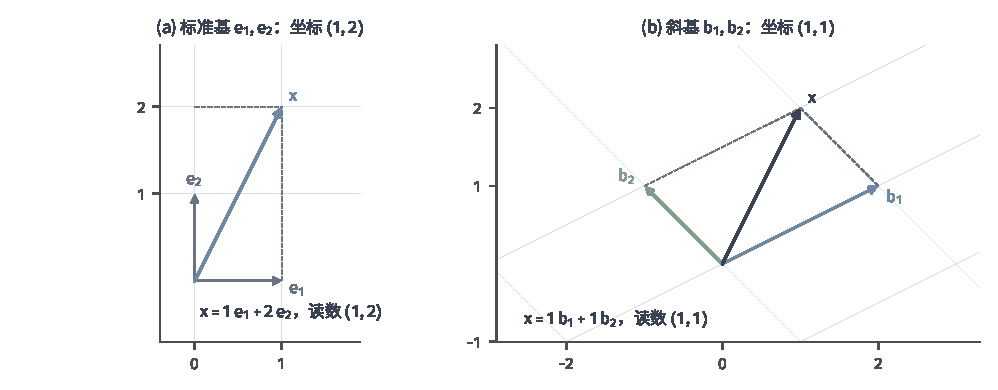
\includegraphics[width=169mm]{figures/00-shared/mathematical-preliminaries-upper/02-linear-spaces/matplotlib/ls-basis-coordinates/ls-basis-coordinates.pdf}
  \caption{同一向量在两组基下的坐标。左：标准基$\bm e_1,\bm e_2$（灰箭头）下，向量$\bm x=(1,2)$（蓝箭头）的坐标为$(1,2)$，虚线为向坐标轴的垂线。右：斜基$\bm b_1=(2,1)$（蓝）、$\bm b_2=(-1,1)$（绿）下，同一个$\bm x$满足$\bm x=\bm b_1+\bm b_2$，坐标为$(1,1)$，浅色斜线为斜基网格，虚线为平行四边形读法。两图坐标系相同。}
  \label{fig:ls-basis-coordinates}
\end{figure*}

\paragraph{坐标与对象}
坐标列要与它所记录的对象区分开：几何位移、有限信号、多项式都可以相加和缩放，它们是\emph{对象}；一列实数只是选定基以后记录对象的\emph{坐标}。基的顺序也要固定：交换$\bm b_1,\bm b_2$，对象不变，坐标列的前两个数也随之交换。在$\mathbb R^d$中直接写数字列，通常是默认使用标准基$\bm e_1,\ldots,\bm e_d$，这时对象与坐标恰好是同一列数，第~\ref{chap:linear-operations}章正是在这种默认下工作的。

函数的基展开则必须区分二者：函数是对象，展开系数是坐标。
\begin{example}[仿射函数在两组基下的坐标]
\label{ex:ls-affine-function-coordinates}
给定：$P_1$中的$f_{a,b}=a+bt$，以及两组基$\mathcal B_1=(1,t)$与$\mathcal B_2=(1,1+t)$。

计算：在$\mathcal B_1$下$f_{a,b}=a\cdot1+b\cdot t$，坐标为$(a,b)^\top$。在$\mathcal B_2$下设$f_{a,b}=c_1\cdot1+c_2(1+t)=(c_1+c_2)+c_2t$，比较常数项与$t$的系数，得$c_2=b$、$c_1=a-b$，即
\[
 f_{a,b}=(a-b)\cdot1+b\cdot(1+t).
\]

结论：同一个函数在$\mathcal B_1$与$\mathcal B_2$下的坐标分别是$(a,b)^\top$与$(a-b,b)^\top$；坐标改变了，函数本身没有改变。
\end{example}
坐标的个数总是维数。一个对象若用冗余的生成组记录，记录的长度可以超过维数，所以不能由这种记录的长度推断空间有几维。

\paragraph{坐标对基的敏感性}
对象不变时，坐标仍可能相差很大。贯穿例给出一个数值上很极端的情形。
\begin{example}[近共线基下的大坐标]
\label{ex:ls-coordinate-instability}
给定：示例~\ref{ex:ls-nearly-collinear-independence}中的$\bm c_1,\bm q$与$\bm c_2=\bm c_1+\varepsilon\bm q$（$\varepsilon\neq0$），$\delta=0.1$，以及目标向量
\begin{equation}
 \bm y=\bm c_1+\delta\bm q=\begin{bmatrix}1\\1.1\\0.9\end{bmatrix}.
 \label{eq:linear-algebra-nearly-collinear-target}
\end{equation}
由该示例，$\mathcal B_0=(\bm c_1,\bm q)$与$\mathcal B_\varepsilon=(\bm c_1,\bm c_2)$都是平面$\operatorname{span}\{\bm c_1,\bm q\}$的基，$\bm y$也在这个平面中。

计算：在$\mathcal B_0$下，$\bm y$的坐标是$(1,\delta)^{\top}$。在$\mathcal B_\varepsilon$下，把$\bm q=(\bm c_2-\bm c_1)/\varepsilon$代入$\bm y=\bm c_1+\delta\bm q$，得
\begin{equation}
 \bm y=\left(1-\frac{\delta}{\varepsilon}\right)\bm c_1
       +\frac{\delta}{\varepsilon}\bm c_2.
 \label{eq:linear-algebra-coordinate-instability}
\end{equation}
取$\varepsilon=0.01$，则$\delta/\varepsilon=10$，坐标成为$(-9,10)^{\top}$。

结论：同一个$\bm y$在$\mathcal B_0$下的坐标为$(1,0.1)^\top$，在$\mathcal B_{0.01}$下的坐标为$(-9,10)^\top$。
\end{example}
两个很大的系数在几乎同向的两个基向量上相互抵消，不能据此判断原对象很大。这种系数对接近退化的基的敏感，将在第~\ref{chap:linear-analysis}章定量讨论。新旧坐标之间怎样系统地换算，是下面要回答的问题。

\paragraph{换基矩阵}
\phantomsection
\label{sec:ls-change-basis}
\label{sec:linear-algebra-coordinate-conversions}
设$\mathcal B=(\bm b_1,\ldots,\bm b_d)$与$\mathcal C$是$V$的两组有序基。已知$\bm v$在$\mathcal B$下的坐标$[\bm v]_{\mathcal B}=(x_1,\ldots,x_d)^{\top}$，怎样求它在$\mathcal C$下的坐标？由$\bm v=\sum_jx_j\bm b_j$，并且坐标映射保持线性组合，
\[
 [\bm v]_{\mathcal C}=\sum_{j=1}^d x_j[\bm b_j]_{\mathcal C}.
\]
右边是各列$[\bm b_j]_{\mathcal C}$以$x_j$为权重的线性组合。把这些列排成矩阵，称为从$\mathcal B$到$\mathcal C$的换基矩阵$\bm S_{\mathcal C\leftarrow\mathcal B}$，按矩阵与向量乘积的列读法，
\begin{equation}
 [\bm v]_{\mathcal C}
 =\bm S_{\mathcal C\leftarrow\mathcal B}[\bm v]_{\mathcal B}.
 \label{eq:linear-algebra-coordinate-change}
\end{equation}
换基矩阵的第$j$列是旧基向量$\bm b_j$的新坐标；下标$\mathcal C\leftarrow\mathcal B$从右向左读，表示把$\mathcal B$坐标译成$\mathcal C$坐标。下面在平面上算一个具体的换基矩阵。
\begin{example}[平面上的换基矩阵]
\label{ex:ls-change-of-basis-plane}
给定：$\mathbb R^2$的标准基$\mathcal E$与基$\mathcal U=(\bm u_1,\bm u_2)$，$\bm u_1=(1,0)^{\top}$、$\bm u_2=(1,1)^{\top}$；向量$\bm v$在$\mathcal U$下的坐标为$(1,1)^\top$。

计算：$\bm u_1,\bm u_2$的标准坐标就是它们自己。按“第$j$列是旧基向量的新坐标”，
\[
 \bm S_{\mathcal E\leftarrow\mathcal U}=\begin{bmatrix}1&1\\0&1\end{bmatrix}.
\]
由式~\eqref{eq:linear-algebra-coordinate-change}，$[\bm v]_{\mathcal E}=\bm S_{\mathcal E\leftarrow\mathcal U}(1,1)^{\top}=(2,1)^{\top}$。直接核对：$\bm v=\bm u_1+\bm u_2=(2,1)^\top$。

结论：$\mathcal U$坐标$(1,1)^\top$与标准坐标$(2,1)^\top$记录的是同一个向量。
\end{example}
图~\ref{fig:vol1-add-linear-change-basis}画出这一点：目标位置没有移动，改变的只是沿哪两条基方向累加，以及每条方向取多少份。
\begin{figure}[!htb]
  \centering
  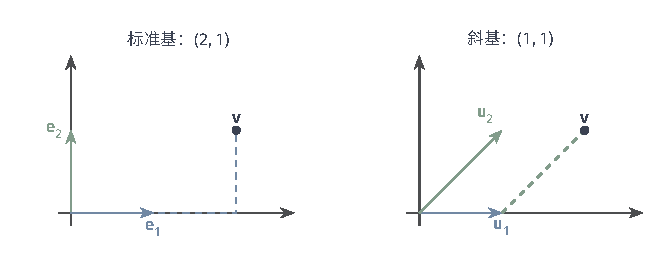
\includegraphics[width=112mm]{figures/00-shared/mathematical-preliminaries-upper/02-linear-spaces/tikz/comprehension-additions/linear-change-basis.pdf}
  \caption{同一向量的两套坐标。左图使用标准基，$\bm v=(2,1)^{\top}$的坐标为$(2,1)^{\top}$；右图使用$\bm u_1=(1,0)^{\top}$、$\bm u_2=(1,1)^{\top}$，同一$\bm v$的坐标为$(1,1)^{\top}$。虚线表示相应的向量相加，两图的环境坐标比例相同。}
  \label{fig:vol1-add-linear-change-basis}
\end{figure}

\paragraph{连续换基与反向换基}
若再换到第三组基$\mathcal D$，中间那套坐标应当不留痕迹。对每个$\bm v$，连用两次式~\eqref{eq:linear-algebra-coordinate-change}，
\[
 [\bm v]_{\mathcal D}=\bm S_{\mathcal D\leftarrow\mathcal C}[\bm v]_{\mathcal C}=\bm S_{\mathcal D\leftarrow\mathcal C}\bm S_{\mathcal C\leftarrow\mathcal B}[\bm v]_{\mathcal B}.
\]
取$\bm v=\bm b_j$，它的$\mathcal B$坐标是$\bm e_j$，两边读出的分别是$\bm S_{\mathcal D\leftarrow\mathcal B}$与乘积的第$j$列，所以
\[
 \bm S_{\mathcal D\leftarrow\mathcal B}
 =\bm S_{\mathcal D\leftarrow\mathcal C}\bm S_{\mathcal C\leftarrow\mathcal B}.
\]

特别取$\mathcal D=\mathcal B$。每个$\bm b_j$在$\mathcal B$下的坐标是$\bm e_j$，所以左边$\bm S_{\mathcal B\leftarrow\mathcal B}=\bm I_d$，即$\bm S_{\mathcal B\leftarrow\mathcal C}\bm S_{\mathcal C\leftarrow\mathcal B}=\bm I_d$；交换两组基的角色，同理得$\bm S_{\mathcal C\leftarrow\mathcal B}\bm S_{\mathcal B\leftarrow\mathcal C}=\bm I_d$。所以换基矩阵总可逆，反向换基矩阵就是它的逆：$\bm S_{\mathcal B\leftarrow\mathcal C}=\bm S_{\mathcal C\leftarrow\mathcal B}^{-1}$。在示例~\ref{ex:ls-change-of-basis-plane}中，$\bm S_{\mathcal U\leftarrow\mathcal E}=\bm S_{\mathcal E\leftarrow\mathcal U}^{-1}=\left[\begin{smallmatrix}1&-1\\0&1\end{smallmatrix}\right]$，它把$(2,1)^{\top}$送回$(1,1)^{\top}$。

反过来，任一$d$阶可逆矩阵$\bm P$都是某次换基的矩阵。以$\bm P$的第$j$列为$\mathcal B$坐标，取向量$\bm b'_j=\sum_i\bm P_{i,j}\bm b_i$。$\bm P$的列线性无关，而坐标映射是保持线性组合的双射，所以$\bm b'_1,\ldots,\bm b'_d$也线性无关。个数等于维数的线性无关组必是基：否则它还能扩充，得到多于$\dim V$个线性无关的向量，与交换引理矛盾。于是$\bm b'_1,\ldots,\bm b'_d$构成一组基$\mathcal B'$。按定义，$\bm S_{\mathcal B\leftarrow\mathcal B'}$的第$j$列是$\bm b'_j$的$\mathcal B$坐标，即$\bm P$的第$j$列，所以$\bm S_{\mathcal B\leftarrow\mathcal B'}=\bm P$。

反向换基的代价取决于换基矩阵是否接近不可逆。贯穿例把这一点表现得很清楚。
\begin{example}[近共线基之间的换基]
\label{ex:ls-nearly-collinear-change-of-basis}
给定：示例~\ref{ex:ls-coordinate-instability}中的两组基$\mathcal B_0=(\bm c_1,\bm q)$与$\mathcal B_\varepsilon=(\bm c_1,\bm c_2)$，$\varepsilon\neq0$。

计算：由$\bm c_1=1\cdot\bm c_1+0\cdot\bm q$与$\bm c_2=1\cdot\bm c_1+\varepsilon\bm q$，$\mathcal B_\varepsilon$的两个向量在$\mathcal B_0$下的坐标分别是$(1,0)^{\top}$与$(1,\varepsilon)^{\top}$，所以
\[
\begin{gathered}
\bm S_{\mathcal B_0\leftarrow\mathcal B_\varepsilon}
 =\begin{bmatrix}1&1\\0&\varepsilon\end{bmatrix}\\
\bm S_{\mathcal B_\varepsilon\leftarrow\mathcal B_0}
 =\bm S_{\mathcal B_0\leftarrow\mathcal B_\varepsilon}^{-1}
 =\begin{bmatrix}1&-1/\varepsilon\\0&1/\varepsilon\end{bmatrix},
\end{gathered}
\]
后者可由直接相乘验证。把$\bm y$在$\mathcal B_0$下的坐标$(1,\delta)^{\top}$代入后者，得
\[
 \bm S_{\mathcal B_\varepsilon\leftarrow\mathcal B_0}\begin{bmatrix}1\\\delta\end{bmatrix}
 =\begin{bmatrix}1-\delta/\varepsilon\\\delta/\varepsilon\end{bmatrix},
\]
与式~\eqref{eq:linear-algebra-coordinate-instability}一致。

结论：$\bm S_{\mathcal B_0\leftarrow\mathcal B_\varepsilon}$的行列式为$\varepsilon$，接近零；反向换基矩阵含有因子$1/\varepsilon$，小的基差异由此被放大成大系数。
\end{example}

\paragraph{被动换基与主动作用}
被动换基与主动作用必须分开。换基时对象不动、记录改变，式\eqref{eq:linear-algebra-coordinate-change}两侧是同一个$\bm v$的两套坐标；主动作用则在固定的坐标下把对象送到另一个对象，例如第~\ref{chap:linear-operations}章的矩阵作用$\bm x\mapsto\bm A\bm x$把向量旋转或切变，下一节把它推广为线性映射。

两者都写成矩阵乘以坐标列，形式相似，含义不同。下面的例子在同一个初始向量上比较两种情形。
\begin{example}[被动换基与主动切变]
\label{ex:ls-passive-vs-active}
给定：$\mathbb R^2$中的向量$\bm x=(3,3)^\top$，斜基$\mathcal B'=(\bm b_1,\bm b_2)$，$\bm b_1=(2,1)^\top$、$\bm b_2=(-1,1)^\top$，以及切变矩阵$\bm A=\left[\begin{smallmatrix}1&1\\0&1\end{smallmatrix}\right]$。

计算：被动换基时，求$\bm x$在$\mathcal B'$下的坐标$(c_1,c_2)^\top$。由$2c_1-c_2=3$与$c_1+c_2=3$得$c_1=2$、$c_2=1$，即$\bm x=2\bm b_1+\bm b_2$。主动作用时，计算$\bm A\bm x=(3+3,\ 3)^\top=(6,3)^\top$。

结论：前者中向量仍是$(3,3)^\top$，只是读数从$(3,3)$变成$(2,1)$；后者中坐标系不动，向量本身被搬到$(6,3)^\top$。
\end{example}
图~\ref{fig:ls-passive-change-vs-active-map}把两种情形并排画出。所以不能把所有乘矩阵的运算都理解成换基。
\begin{figure*}[htbp]
  \centering
  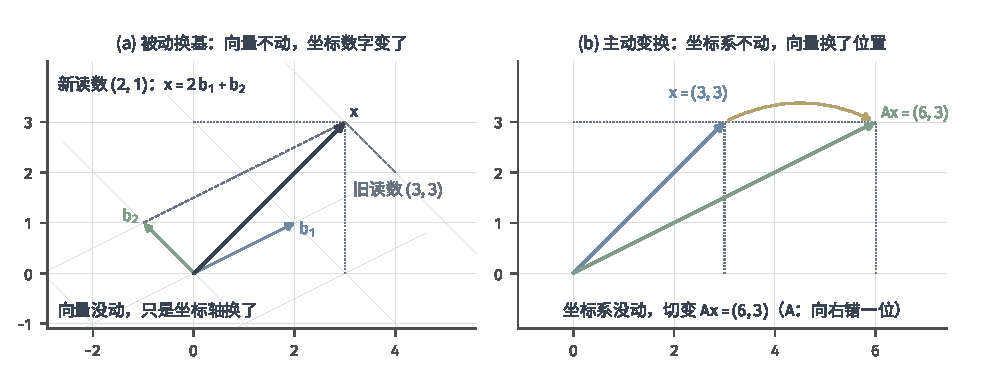
\includegraphics[width=169mm]{figures/00-shared/mathematical-preliminaries-upper/02-linear-spaces/matplotlib/ls-passive-change-vs-active-map/ls-passive-change-vs-active-map.pdf}
  \caption{被动换基与主动变换的对照，两图使用同一个初始向量$\bm x=(3,3)$。左（被动换基）：箭头位置不动（深色），旧标准读数用点线投影读出$(3,3)$；新斜基$\bm b_1=(2,1)$（蓝）、$\bm b_2=(-1,1)$（绿）与浅色斜网格下，$\bm x=2\bm b_1+\bm b_2$，新读数为$(2,1)$。右（主动变换）：标准坐标系不动，$\bm x$（蓝）被切变映到$\bm A\bm x=(6,3)$（绿），黄色弧线表示搬动过程。}
  \label{fig:ls-passive-change-vs-active-map}
\end{figure*}

% 第5章第3节：线性映射（定义；表示：矩阵表示、基于矩阵的映射运算、矩阵基本子空间；核与像、秩零度、商空间、行空间与列空间、可逆性；换基：相抵与相似）。

\section{线性与多线性映射}
\label{sec:ls-linear-maps}
\label{sec:linear-algebra-matrices-linear-maps}

前两节研究的是单个空间中的对象怎样记录；本节转向对象之间的作用。一个作用要满足什么条件，才能用前两节的语言处理？选定基以后，它怎样记录成一张数表，两个作用叠加或接连进行时数表怎样变化？作用保留了哪些输入信息、丢失了哪些，什么时候可以由输出唯一反求输入？换一组基，记录同一个作用的数表怎样改变，哪些量不随之改变？本节的四个小节依次回答这四个问题。

\subsection{线性映射及其矩阵表示}
\label{sec:ls-linear-map-definition}
\label{sec:linear-algebra-maps}

设计矩阵把一组系数变成一列拟合值，求导把一个多项式变成另一个多项式，读取第一个坐标把向量变成一个数。这些作用有一个共同点：输入先加权相加再作用，与先分别作用再作同样的加权相加，结果相同。正是这一点让前两节的语言可以用于作用本身：输入写成基向量的组合，作用就可以逐个基向量地计算。保持线性组合的作用称为\term{线性映射}（linear map）$T:V\to W$：
\begin{equation}
\begin{gathered}
T(a\bm x+b\bm y)=aT\bm x+bT\bm y\\
\bm x,\bm y\in V,\ a,b\in\mathbb R.
\end{gathered}
\label{eq:ls-linear-map-def}
\end{equation}
取$a=b=0$得$T\bm0=\bm0$，线性映射总把原点留在原处。由式~\eqref{eq:prelim-matrix-linearity}，任何矩阵$\bm A\in\mathbb R^{m\times d}$给出的$\bm x\mapsto\bm A\bm x$都是从$\mathbb R^d$到$\mathbb R^m$的线性映射。下面再检查几个作用是否线性。
\begin{example}[线性与非线性的作用]
\label{ex:ls-linear-map-checks}
给定：三个作用
\[
 \begin{aligned}
 &T:\mathbb R^2\to\mathbb R^2, &&T(x_1,x_2)=(2x_1+x_2,\ 3x_2);\\
 &D:P_k\to P_k, &&Dp=p';\\
 &\tau:\mathbb R\to\mathbb R, &&\tau(x)=x+1.
 \end{aligned}
\]

验证：$T(x_1,x_2)$就是$\left[\begin{smallmatrix}2&1\\0&3\end{smallmatrix}\right]\bm x$，所以$T$保持线性组合。对多项式有$(ap+bq)'=ap'+bq'$，所以$D$保持线性组合；求导不升高次数，$D$确实把$P_k$送回$P_k$。$\tau(0)=1\neq0$，而线性映射必把$0$送到$0$。

结论：$T$与$D$是线性映射，$\tau$不是线性映射。
\end{example}

\phantomsection
\label{sec:ls-operator-powers}
输入与输出是同一个空间的线性映射$T:V\to V$称为\term{线性算子}（linear operator），也称线性变换。平面上的旋转、向一条直线的投影、$P_k$上的求导都是线性算子，示例~\ref{ex:ls-linear-map-checks}中的$T$也是。

算子是映射的特殊情形，但这一限制带来两点实质的不同。第一，输出仍在$V$中，可以再次作为输入，所以算子能与自身复合、反复作用：记$T^2=T\circ T$、$T^k=T\circ T^{k-1}$，并约定$T^0=\operatorname{id}_V$；一般映射$V\to W$在$V\neq W$时不能这样反复作用。下面将看到，在同一组基下，$T^k$的矩阵就是$T$的矩阵的$k$次幂。

第二，记录算子时输入、输出可以用同一组基，这决定了算子换基时的特殊规律（第~\ref{sec:ls-similarity}节）。

\paragraph{坐标表示与运算}
\label{sec:ls-map-representation}

线性映射的定义域通常有无穷多个元素，逐个记录输出是不可能的。本小节说明，有了基，有限个数就够了：在固定的两组基下，线性映射与矩阵一一对应，映射的叠加、复合与求逆分别对应矩阵的加法、乘法与求逆。第~\ref{chap:linear-operations}章的矩阵运算由此获得一般含义：矩阵就是线性映射在坐标下的记录。下面先建立这一对应，再把映射的运算翻译成矩阵的运算，最后对矩阵定义四个基本子空间，供下一小节计数信息的丢失与保留。

\subsubsection{矩阵表示}

给定输入基$\mathcal B=(\bm b_1,\ldots,\bm b_d)$，任一$\bm v=\sum_jx_j\bm b_j$的像由线性性写成
\[
 T\bm v=\sum_{j=1}^d x_j\,T\bm b_j,
\]
所以只要知道$d$个基向量的像，整个映射就确定了。再给定输出基$\mathcal C$，把每个像的坐标$[T\bm b_j]_{\mathcal C}$作为第$j$列，排成矩阵$\bm A=[T]_{\mathcal C\leftarrow\mathcal B}\in\mathbb R^{m\times d}$，称为$T$在这两组基下的矩阵。对上式两边取$\mathcal C$坐标，由坐标映射保持线性组合，并按矩阵与向量乘积的列读法，得到
\begin{equation}
 [T\bm v]_{\mathcal C}
 =\sum_{j=1}^d x_j\,[T\bm b_j]_{\mathcal C}
 =\sum_{j=1}^d x_j\bm A_{:,j}
 =[T]_{\mathcal C\leftarrow\mathcal B}\,[\bm v]_{\mathcal B}.
 \label{eq:linear-algebra-map-matrix-representation}
\end{equation}
也就是说，输出坐标等于矩阵乘以输入坐标：作用在对象上进行，记录在坐标上进行，二者由矩阵与向量的乘积连接。列数是输入维数，行数是输出维数；下标$\mathcal C\leftarrow\mathcal B$从右向左读，表示输入用$\mathcal B$记录、输出用$\mathcal C$记录。输入输出为同一空间的算子通常两端用同一组基，记为$[T]_{\mathcal B}=[T]_{\mathcal B\leftarrow\mathcal B}$，它是$\dim V$阶方阵。

下面按这一规则写出两个映射的矩阵。
\begin{example}[由基向量的像写出矩阵]
\label{ex:ls-plane-operator-matrix}
给定：示例~\ref{ex:ls-linear-map-checks}中的$T(x_1,x_2)=(2x_1+x_2,\ 3x_2)$，输入输出都取标准基。

计算：$T\bm e_1=(2,0)^{\top}$，$T\bm e_2=(1,3)^{\top}$。把它们依次作为两列，得
\[
 [T]=\begin{bmatrix}2&1\\0&3\end{bmatrix}.
\]

结论：$[T]$正是定义$T$时用的矩阵。
\end{example}
一般地，$\bm x\mapsto\bm A\bm x$在标准基下的矩阵就是$\bm A$本身，因为$\bm A\bm e_j=\bm A_{:,j}$。矩阵表示同样适用于不是数组的对象。
\begin{example}[求导的矩阵表示]
\label{ex:ls-derivative-matrix}
给定：求导$D:P_2\to P_2$，输入输出都取基$(1,t,t^2)$。

计算：$D1=0$，$Dt=1$，$Dt^2=2t$，三个像的坐标依次为$(0,0,0)^\top$、$(1,0,0)^\top$、$(0,2,0)^\top$，所以
\[
 [D]=\begin{bmatrix}0&1&0\\0&0&2\\0&0&0\end{bmatrix}.
\]
多项式$p=a_0+a_1t+a_2t^2$的坐标是$(a_0,a_1,a_2)^\top$，而$[D](a_0,a_1,a_2)^\top=(a_1,2a_2,0)^\top$，正是$p'=a_1+2a_2t$的坐标。

结论：对函数求导，在坐标下就是乘矩阵$[D]$。
\end{example}

\begin{theorem}[线性映射与矩阵的对应]
\label{thm:ls-map-matrix-correspondence}
设$\dim V=d$、$\dim W=m$，并固定$V$的基$\mathcal B$与$W$的基$\mathcal C$。则$T\mapsto[T]_{\mathcal C\leftarrow\mathcal B}$是从全部线性映射$V\to W$到全部$m\times d$实矩阵的双射。
\end{theorem}
\begin{proof}
单射：若两个线性映射的矩阵相同，它们在每个基向量上的像相同，由$T\bm v=\sum_jx_jT\bm b_j$，它们在每个$\bm v$上都相同。满射：任给$\bm A\in\mathbb R^{m\times d}$，对$\bm v\in V$令$T\bm v$为$\mathcal C$坐标等于$\bm A[\bm v]_{\mathcal B}$的那个向量。坐标唯一，所以这一规则有确定的意义；坐标映射与乘矩阵都保持线性组合，所以$T$线性；$T\bm b_j$的坐标是$\bm A\bm e_j=\bm A_{:,j}$，所以$[T]_{\mathcal C\leftarrow\mathcal B}=\bm A$。
\end{proof}
所以基固定以后，线性映射与矩阵一一对应；每个从$\mathbb R^d$到$\mathbb R^m$的线性映射在标准基下都等于乘某个矩阵。不过这一对应依赖基的选取：改变两端任一组基，通常会改变数表，而数表记录的仍是同一个映射。数表具体怎样随基改变，在第~\ref{sec:ls-coordinates-change-of-basis}节推导。

设计矩阵$\bm X_\varepsilon$正是这样一张记录：它表示$T_\varepsilon:\mathbb R^2\to\mathbb R^3$，$\bm w\mapsto\bm X_\varepsilon\bm w=w_1\bm c_1+w_2\bm c_2$，两列分别是两个输入基向量的像。输入是两个系数，输出是三个样本的拟合值，二者不能当成同一个空间中的向量。矩阵只是映射在两端坐标下的记录，不是映射本身的全部含义。图~\ref{fig:ch06-object-coordinate-map}中两条路径给出同一结果：先作用于对象再取坐标，与先取输入坐标再乘矩阵，得到相同的输出坐标。
\begin{figure}[htbp]
  \centering
  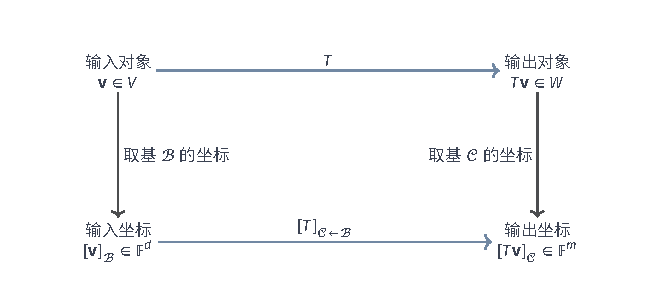
\includegraphics[width=112.0mm]{figures/00-shared/mathematical-preliminaries-upper/02-linear-spaces/tikz/ch06-object-coordinate-map/figure.pdf}
  \caption{先作用于对象再取坐标，与先取输入坐标再按矩阵的列作线性组合（即乘矩阵），得到相同输出坐标。横向箭头改变对象或数值，竖向箭头只改变记录方式。}
  \label{fig:ch06-object-coordinate-map}
\end{figure}

\subsubsection{基于矩阵的映射运算}
\phantomsection
\label{sec:ls-map-addition-composition}

两个映射可以把输出相加，也可以接连作用；一个映射可能可以撤销，也可能带上常数偏置。第~\ref{chap:linear-operations}章的矩阵加法、乘法与求逆，正是前三种运算在固定基下的记录；带偏置的仿射映射则可以借增广坐标写成一张更大的矩阵。

\paragraph{叠加}
\phantomsection
\label{sec:linear-algebra-map-addition}
设$T,S:V\to W$是同一对空间之间的两个线性映射，定义
\[
\begin{gathered}
(aT+bS)(\bm x)=aT\bm x+bS\bm x\\
\bm x\in V,
\end{gathered}
\]
其中$a,b\in\mathbb R$。叠加保持线性：把输入的线性组合代入，两个分支分别展开再汇总即可。在$V$与$W$的固定基下，若$T,S$的矩阵为$\bm A,\bm B$，则$aT+bS$把第$j$个基向量送到$aT\bm b_j+bS\bm b_j$，其坐标是$a\bm A_{:,j}+b\bm B_{:,j}$，所以$aT+bS$的矩阵就是$a\bm A+b\bm B$。

相加的前提是两个映射的定义域与陪域都一致。这并不要求$V=W$：两个从$\mathbb R^2$到$\mathbb R^3$的映射照样可以相加，只是不能与一个从$\mathbb R^3$到$\mathbb R^2$的映射相加；这对应于只有同形矩阵才能相加。系数$a,b$必须与输入无关；若叠加系数随$\bm x$改变，叠加后的映射一般不再线性，需要单独检验。

\paragraph{复合}
设$T:U\to V$、$S:V\to W$是线性映射。复合$S\circ T$先$T$后$S$，仍保持线性组合：$S(T(a\bm x+b\bm y))=S(aT\bm x+bT\bm y)=aS(T\bm x)+bS(T\bm y)$。取$U,V,W$的基$\mathcal B,\mathcal C,\mathcal D$，对每个$\bm x\in U$，两次使用式~\eqref{eq:linear-algebra-map-matrix-representation}，再用矩阵乘法的结合律，得
\[
 [S(T\bm x)]_{\mathcal D}
 =[S]_{\mathcal D\leftarrow\mathcal C}[T\bm x]_{\mathcal C}
 =[S]_{\mathcal D\leftarrow\mathcal C}\bigl([T]_{\mathcal C\leftarrow\mathcal B}[\bm x]_{\mathcal B}\bigr)
 =\bigl([S]_{\mathcal D\leftarrow\mathcal C}[T]_{\mathcal C\leftarrow\mathcal B}\bigr)[\bm x]_{\mathcal B}.
\]
取$\bm x=\bm b_j$，其坐标是$\bm e_j$，两边读出的是$[S\circ T]_{\mathcal D\leftarrow\mathcal B}$与乘积的第$j$列，所以
\begin{equation}
 [S\circ T]_{\mathcal D\leftarrow\mathcal B}
 =[S]_{\mathcal D\leftarrow\mathcal C}\,[T]_{\mathcal C\leftarrow\mathcal B}.
 \label{eq:ls-composition-matrix}
\end{equation}

复合的矩阵是矩阵的乘积，中间空间$V$的基$\mathcal C$在乘积中被消去；第~\ref{sec:prelim-linear-actions-composition}节的推导是这里取标准基的特例。恒等映射$\operatorname{id}_V$在同一组基下的矩阵是单位矩阵。于是映射复合的结合律与矩阵乘法的结合律互相对应，矩阵乘法不可交换，也就是先后作用的次序不能交换。

对算子$T:V\to V$两端都用基$\mathcal B$，反复使用式~\eqref{eq:ls-composition-matrix}，得$[T^k]_{\mathcal B}=([T]_{\mathcal B})^k$：算子的反复作用记录为第~\ref{sec:ls-matrix-power-rules}节的矩阵幂。例如对示例~\ref{ex:ls-derivative-matrix}中的$[D]$直接相乘可得$[D]^3=\bm0$，这对应于任何次数不超过$2$的多项式求导三次都变为零。

\paragraph{逆映射}
第~\ref{sec:prelim-inverse-matrices}节把满足$\bm A\bm B=\bm B\bm A=\bm I$的方阵$\bm A$称为可逆矩阵，那里只把它看成一次可以撤销的数表运算。有了矩阵表示，就可以问它记录的是哪一类映射。若线性映射$T:V\to W$是双射（第~\ref{chap:sets-functions-and-proofs}章~\ref{sec:prelim-function-types}节），每个输出恰有一个原输入，逆映射$T^{-1}:W\to V$存在。逆映射自动是线性的：对$\bm w,\bm w'\in W$，由$T$的线性性
\[
 T\bigl(aT^{-1}\bm w+bT^{-1}\bm w'\bigr)=a\bm w+b\bm w',
\]
所以$aT^{-1}\bm w+bT^{-1}\bm w'$就是$a\bm w+b\bm w'$唯一的原输入，即$T^{-1}(a\bm w+b\bm w')=aT^{-1}\bm w+bT^{-1}\bm w'$。这样的$T$称为可逆线性映射。

可逆映射与可逆矩阵是同一件事的两种记录。

设$T:V\to W$可逆，在基$\mathcal B,\mathcal C$下$\bm A=[T]_{\mathcal C\leftarrow\mathcal B}$，$\bm B=[T^{-1}]_{\mathcal B\leftarrow\mathcal C}$。由式~\eqref{eq:ls-composition-matrix}，$T^{-1}\circ T=\operatorname{id}_V$与$T\circ T^{-1}=\operatorname{id}_W$分别给出$\bm B\bm A=\bm I$与$\bm A\bm B=\bm I$，所以$\bm A$是可逆方阵（下一小节将说明此时必有$\dim V=\dim W$），且$[T^{-1}]_{\mathcal B\leftarrow\mathcal C}=\bm A^{-1}$。反过来，若$\bm A$可逆，$\bm y\mapsto\bm A^{-1}\bm y$就是$\bm x\mapsto\bm A\bm x$的逆映射。

两个可逆映射接连作用时，$(S\circ T)^{-1}=T^{-1}\circ S^{-1}$，在矩阵上就是式~\eqref{eq:ls-inverse-product}。至于一个映射什么时候可逆，要先弄清它丢失了什么、能到达什么，这是下一小节的内容。

\paragraph{仿射映射}
\phantomsection
\label{sec:ls-affine-maps}
线性模型的预测常带截距，平面上的平移也常与旋转一起出现，它们都不把原点留在原处。这样的作用怎样纳入线性映射的框架？带常数偏置的规则$\bm x\mapsto\bm A\bm x+\bm b$称为\term{仿射映射}（affine map）。当$\bm b\neq\bm0$时，它不是线性映射：它把$\bm0$送到$\bm b$，而线性映射必将$\bm0$送到$\bm0$。当$\bm b=\bm0$时，它就是线性映射。

两个仿射映射$\bm x\mapsto\bm A_1\bm x+\bm b_1$、$\bm y\mapsto\bm A_2\bm y+\bm b_2$复合得$\bm x\mapsto\bm A_2\bm A_1\bm x+(\bm A_2\bm b_1+\bm b_2)$，前一个映射的平移项也被后一个映射作用。

给坐标补一个恒为$1$的末位，仿射映射可以写成高一维空间上的线性作用：
\begin{equation}
 \begin{bmatrix}\bm A&\bm b\\ \bm0^\top&1\end{bmatrix}
 \begin{bmatrix}\bm x\\1\end{bmatrix}
 =
 \begin{bmatrix}\bm A\bm x+\bm b\\1\end{bmatrix}.
 \label{eq:ls-affine-homogeneous}
\end{equation}
按分块乘法，两个这样的增广矩阵相乘得
\[
 \begin{bmatrix}\bm A_2&\bm b_2\\ \bm0^\top&1\end{bmatrix}
 \begin{bmatrix}\bm A_1&\bm b_1\\ \bm0^\top&1\end{bmatrix}
 =\begin{bmatrix}\bm A_2\bm A_1&\bm A_2\bm b_1+\bm b_2\\ \bm0^\top&1\end{bmatrix},
\]
正是复合仿射映射的增广矩阵。

大矩阵对整个增广空间是线性的，但原输入被限制在末坐标为$1$的集合上，不能据此声称原映射线性。第~\ref{chap:linear-equations-and-optimization}章用这种形式描述仿射解集的几何。

\subsubsection{矩阵基本子空间}
\phantomsection
\label{sec:ls-four-fundamental-subspaces}

一张矩阵$\bm A\in\mathbb R^{m\times d}$既给出从$\mathbb R^d$到$\mathbb R^m$的映射$\bm x\mapsto\bm A\bm x$，它的转置$\bm A^\top\in\mathbb R^{d\times m}$又给出反方向的映射$\bm y\mapsto\bm A^\top\bm y$。对每个方向问两个问题：哪些输出可以到达，哪些输入被送到零。四个答案都是子空间，它们刻画了矩阵怎样保留和丢失信息。

按矩阵与向量乘积的列读法，$\bm A\bm x=\sum_jx_j\bm A_{:,j}$；$\bm x$取遍$\mathbb R^d$时，输出取遍$\bm A$各列的全部线性组合，即各列的张成空间，称为$\bm A$的\term{列空间}（column space），记为$\operatorname{range}(\bm A)$。所以方程$\bm A\bm x=\bm b$有解当且仅当$\bm b\in\operatorname{range}(\bm A)$。

齐次方程组$\bm A\bm x=\bm0$的解集合是$\mathbb R^d$的子空间（示例~\ref{ex:ls-subspace-checks}），称为$\bm A$的\term{零空间}（null space），记为$\operatorname{null}(\bm A)$。对$\bm A^\top$问同样的两个问题，又得到两个子空间。$\bm A^\top$的列就是$\bm A$的行（竖排），所以$\operatorname{range}(\bm A^\top)$由$\bm A$各行的线性组合组成，称为$\bm A$的\term{行空间}（row space）。$\bm A^\top\bm y=\bm0$转置后就是$\bm y^\top\bm A=\bm0^\top$：$\bm y^\top$从左边乘上$\bm A$得到零，所以$\operatorname{null}(\bm A^\top)$称为$\bm A$的\term{左零空间}（left null space）。这四个子空间合称$\bm A$的\term{四个基本子空间}（four fundamental subspaces）：
\begin{equation}
 \begin{aligned}
  \operatorname{range}(\bm A)&=\{\bm A\bm x:\bm x\in\mathbb R^d\}\subseteq\mathbb R^m,\\
  \operatorname{null}(\bm A)&=\{\bm x\in\mathbb R^d:\bm A\bm x=\bm0\}\subseteq\mathbb R^d,\\
  \operatorname{range}(\bm A^\top)&=\{\bm A^\top\bm y:\bm y\in\mathbb R^m\}\subseteq\mathbb R^d,\\
  \operatorname{null}(\bm A^\top)&=\{\bm y\in\mathbb R^m:\bm A^\top\bm y=\bm0\}\subseteq\mathbb R^m.
 \end{aligned}
 \label{eq:ls-four-fundamental-subspaces}
\end{equation}

零空间与行空间在输入空间$\mathbb R^d$中，列空间与左零空间在输出空间$\mathbb R^m$中。零空间收集被完全消去的输入方向。行空间收集读取输出分量所用的方向：输出的第$i$个分量$(\bm A\bm x)_i=\bm A_{i,:}\bm x$是第$i$行与$\bm x$逐项相乘再相加。左零空间收集对可达输出的“盲读”：对$\bm y\in\operatorname{null}(\bm A^\top)$与任意输入$\bm x$，$\bm y^\top(\bm A\bm x)=(\bm y^\top\bm A)\bm x=0$，即用$\bm y$对可达输出加权求和，结果总是零。

下面对一个具体矩阵求出四个基本子空间。
\begin{example}[一个$2\times3$矩阵的四个基本子空间]
\label{ex:ls-rank-one-four-subspaces}
给定：
\[
 \bm A=\begin{bmatrix}1&2&3\\2&4&6\end{bmatrix}\in\mathbb R^{2\times3}.
\]

计算：列空间：三列$(1,2)^\top$、$(2,4)^\top$、$(3,6)^\top$都是$(1,2)^\top$的倍数，所以$\operatorname{range}(\bm A)=\operatorname{span}\{(1,2)^\top\}$，是$\mathbb R^2$中的直线。零空间：第二行是第一行的$2$倍，$\bm A\bm x=\bm0$只剩一个方程$x_1+2x_2+3x_3=0$，由示例~\ref{ex:ls-solution-plane-basis}，$\operatorname{null}(\bm A)=\operatorname{span}\{(-2,1,0)^\top,(-3,0,1)^\top\}$，是$\mathbb R^3$中的平面。行空间：两行都是$(1,2,3)$的倍数，所以$\operatorname{range}(\bm A^\top)=\operatorname{span}\{(1,2,3)^\top\}$，是$\mathbb R^3$中的直线。左零空间：$\bm y^\top\bm A=(y_1+2y_2)(1,2,3)$为零当且仅当$y_1=-2y_2$，所以$\operatorname{null}(\bm A^\top)=\operatorname{span}\{(2,-1)^\top\}$，是$\mathbb R^2$中的直线。

结论：列空间、零空间、行空间、左零空间的维数依次为$1,2,1,1$。列空间与行空间维数相同；输入空间中零空间与行空间的维数之和为$2+1=3$，输出空间中列空间与左零空间的维数之和为$1+1=2$。此外，行空间的方向$(1,2,3)^\top$与零空间的两个基向量逐项相乘再相加都得零（$-2+2+0=0$，$-3+0+3=0$），列空间的方向$(1,2)^\top$与左零空间的方向$(2,-1)^\top$也是如此（$2-2=0$）。
\end{example}
第~\ref{sec:ls-kernel-image}节说明，示例中的两条维数规律对任何矩阵都成立；垂直关系则要等第~\ref{sec:ls-orthogonality}节有了内积以后才能说清。

\subsection{核、像与秩}
\label{sec:ls-kernel-image}

一个映射丢失了哪些输入信息，又能产生哪些输出？这两个问题决定了能否由输出反求输入。本小节先把它们写成两个子空间，再用秩零度定理说明二者的维数此消彼长，并用商空间重新解读这一关系；然后求出矩阵四个基本子空间的维数；最后给出单射、满射与可逆的判据。

\paragraph{核与像}
被映射送到零的输入集合称为$T$的核（kernel），记为$\ker T=\{\bm x\in V:T\bm x=\bm0\}$；所有可到达的输出集合称为\term{像空间}（简称像，image），记为$\operatorname{im}T=\{T\bm x:\bm x\in V\}$。二者都是子空间：若$T\bm x=T\bm y=\bm0$，则$T(a\bm x+b\bm y)=\bm0$；若$\bm u=T\bm x$、$\bm v=T\bm y$，则$a\bm u+b\bm v=T(a\bm x+b\bm y)$。

核记录被映射完全消去的输入方向，像记录可达的输出范围；二者分别位于输入端与输出端，不能当作同一空间中的两个集合直接比较。对矩阵$\bm A\in\mathbb R^{m\times d}$，映射$\bm x\mapsto\bm A\bm x$的核就是零空间$\operatorname{null}(\bm A)$，像就是列空间$\operatorname{range}(\bm A)$（第~\ref{sec:ls-four-fundamental-subspaces}节）。说“矩阵$\bm A$的核”“矩阵$\bm A$的秩”时，指的都是映射$\bm x\mapsto\bm A\bm x$的相应量。

核为什么代表“丢失的信息”？因为$T\bm x=T\bm y$当且仅当$T(\bm x-\bm y)=\bm0$，即$\bm x-\bm y\in\ker T$：两个输入相差一个核方向时，输出完全相同。下面的例子用三个响应读取四个分量，展示这一点。
\begin{example}[相差核方向的输入给出相同输出]
\label{ex:ls-kernel-indistinguishable}
给定：$T:\mathbb R^4\to\mathbb R^3$，
\[
 T(x_1,x_2,x_3,x_4)=(x_1+x_4,\ x_2+x_4,\ x_3+x_4).
\]

计算：$T\bm x=\bm0$当且仅当$x_1=x_2=x_3=-x_4$，所以$\ker T=\operatorname{span}\{(1,1,1,-1)^{\top}\}$。取$x_4=0$时，$T\bm x=(x_1,x_2,x_3)$可以是任意向量，所以$\operatorname{im}T=\mathbb R^3$。两个输入$(1,1,1,1)^\top$与$(0,0,0,2)^\top$之差为$(1,1,1,-1)^\top\in\ker T$，相应地
\[
 T(1,1,1,1)=T(0,0,0,2)=(2,2,2).
\]

结论：仅凭三个响应无法区分这两个输入，也无法区分任何两个相差$(1,1,1,-1)^\top$倍数的输入。
\end{example}
这就是线性不可辨识性：两个输入相差核方向时输出相同，只凭输出无法确定输入。若另有约束限制了可取的输入，能否辨识还要结合这些约束判断。

\paragraph{秩零度定理}
\phantomsection
\label{sec:ls-rank-nullity}
核与像各有多大？二者的维数之间有一条精确的守恒关系。像的维数称为\term{秩}（rank）$\operatorname{rank}T=\dim\operatorname{im}T$，核的维数称为\term{零度}（nullity）$\dim\ker T$。
\begin{theorem}[秩零度定理]
\label{thm:ls-rank-nullity}
\label{thm:linear-algebra-rank-nullity}
有限维线性映射$T:V\to W$满足
\begin{equation}
\begin{gathered}
\dim V=\dim\ker T+\dim\operatorname{im}T\\
\text{即}\qquad
 \dim V=\dim\ker T+\operatorname{rank}T.
\end{gathered}
\label{eq:ls-rank-nullity}
\end{equation}
\end{theorem}
\begin{proof}
取核的一组基$\bm v_1,\ldots,\bm v_r$并扩充成$V$的基$\bm v_1,\ldots,\bm v_d$。前$r$个基向量的像为零，所以其余像$T\bm v_{r+1},\ldots,T\bm v_d$张成像。若$\sum_{j>r}a_jT\bm v_j=\bm0$，则$\sum_{j>r}a_j\bm v_j$属于核，能由前$r$个基向量表示；整个基的线性无关性迫使全部$a_j=0$，所以这些像也是无关组。像的维数为$d-r$，结论成立。
\end{proof}
对矩阵$\bm A\in\mathbb R^{m\times d}$，记$\operatorname{rank}\bm A$为其映射的秩，即列空间的维数，有$d=\dim\operatorname{null}(\bm A)+\operatorname{rank}\bm A$。秩计数独立的输出方向，零度计数被消去的独立输入方向，二者此消彼长。在示例~\ref{ex:ls-kernel-indistinguishable}中，$\dim\ker T=1$、$\operatorname{rank}T=3$，二者之和为输入维数$4$。图~\ref{fig:ls-kernel-image-rank-nullity}再给出两个几何化算例：被映到零的方向与实际用到的输出方向，维数相加恰为定义域维数。
\begin{figure*}[htbp]
  \centering
  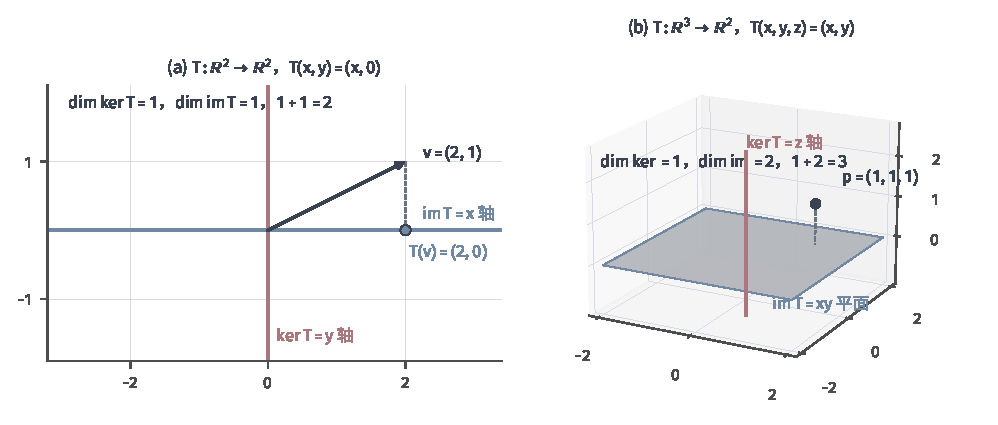
\includegraphics[width=169mm]{figures/00-shared/mathematical-preliminaries-upper/02-linear-spaces/matplotlib/ls-kernel-image-rank-nullity/ls-kernel-image-rank-nullity.pdf}
  \caption{核与像的维数此消彼长。左：$T(x,y)=(x,0)$把平面映到$x$轴，核是$y$轴（红直线）、像是$x$轴（蓝直线），$\dim\ker T=1$、$\dim\operatorname{im}T=1$，$1+1=2$；样本$\bm v=(2,1)$被映到$(2,0)$。右：$T(x,y,z)=(x,y)$把三维空间映到$xy$平面，核是$z$轴（红直线）、像是整个$xy$平面（浅蓝），$\dim\ker T=1$、$\dim\operatorname{im}T=2$，$1+2=3$。两图为解析教学例。}
  \label{fig:ls-kernel-image-rank-nullity}
\end{figure*}

对$\bm A\in\mathbb R^{m\times d}$，$\operatorname{rank}\bm A\leq\min(m,d)$：列空间在$\mathbb R^m$中，维数不超过$m$；它由$d$列张成，从中抽取出的基不超过$d$个向量。$\operatorname{rank}\bm A=d$称为满列秩，这时输入方向全部被保留，等价于各列线性无关；$\operatorname{rank}\bm A=m$称为满行秩，这时输出全部可达；二者统称\term{满秩}（full rank）。

形状不同时，二者不能同时成立。$m<d$时，即使满行秩，核的维数也是$d-m>0$；$m>d$时，即使满列秩，像的维数也只有$d<m$，总有输出无法到达。例如贯穿例$\bm X_\varepsilon$在$\varepsilon\neq0$时两列线性无关（示例~\ref{ex:ls-nearly-collinear-independence}），秩为$2$，满列秩；它的像是$\mathbb R^3$中的一个平面，不是满行秩。

\paragraph{商空间}
前面看到，输出相同的输入恰好彼此相差一个核方向。按输出把输入分组，每组都形如$\bm x+\ker T$，正是第~\ref{sec:ls-quotient-spaces}节取$U=\ker T$得到的等价类，全部分组组成商空间$V/\ker T$。

规则$\bm x+\ker T\mapsto T\bm x$不依赖代表元，因为代表元相差核方向时输出相同。它保持线性组合，满射到$\operatorname{im}T$；它也是单射，因为两个类的像相同即$T\bm x=T\bm y$时，$\bm x-\bm y\in\ker T$，两个类相同。所以它是从$V/\ker T$到$\operatorname{im}T$的线性双射：压去全部丢失方向以后，每个等价类恰对应一个可达输出。线性双射把一组基送到一组基，两边维数相同；由式~\eqref{eq:ls-quotient-dimension}得$\dim V-\dim\ker T=\operatorname{rank}T$，这是秩零度定理的另一种读法。在示例~\ref{ex:ls-kernel-indistinguishable}中，商空间$\mathbb R^4/\ker T$是三维的，像$\mathbb R^3$也是三维的。

\paragraph{矩阵的行空间与列空间}
示例~\ref{ex:ls-rank-one-four-subspaces}中，行空间与列空间维数相同，零空间与行空间的维数之和为输入维数，列空间与左零空间的维数之和为输出维数。现在对一般的$\bm A\in\mathbb R^{m\times d}$证明这些规律。对$\bm A$用秩零度定理，零空间与列空间的维数之和为$d$；对$\bm A^\top$用它，左零空间与行空间的维数之和为$m$。剩下的问题是两个“列空间”之间的关系：行空间与列空间是否总一样大？
\begin{theorem}[行秩等于列秩]
\label{thm:ls-row-rank-column-rank}
对任意$\bm A\in\mathbb R^{m\times d}$，$\dim\operatorname{range}(\bm A^\top)=\dim\operatorname{range}(\bm A)$，即$\operatorname{rank}\bm A^\top=\operatorname{rank}\bm A$。
\end{theorem}
\begin{proof}
设$r=\operatorname{rank}\bm A$，取列空间的一组基$\bm c_1,\ldots,\bm c_r$，排成$\bm C\in\mathbb R^{m\times r}$。$\bm A$的每一列都在列空间中，所以第$j$列可写成$\bm A_{:,j}=\bm C\bm r_j$，$\bm r_j\in\mathbb R^r$；把这些系数列排成$\bm R\in\mathbb R^{r\times d}$，按乘积的列读法得$\bm A=\bm C\bm R$。再按行读这个乘积：$\bm A$的第$i$行是$\bm A_{i,:}=\sum_{k=1}^r\bm C_{i,k}\bm R_{k,:}$，即$\bm R$的$r$行的线性组合。所以$\bm A$的全部行都落在$\bm R$的$r$行张成的空间里，行空间的维数不超过$r$，即$\operatorname{rank}\bm A^\top\leq\operatorname{rank}\bm A$。对$\bm A^\top$用同样的论证，得$\operatorname{rank}\bm A\leq\operatorname{rank}\bm A^\top$，两者相等。
\end{proof}
于是行秩（行空间的维数）与列秩（列空间的维数）可以统称为秩。对$\bm A$与$\bm A^\top$分别用秩零度定理，四个基本子空间的维数全部由$m,d$与$r=\operatorname{rank}\bm A$决定：
\begin{equation}
 \begin{gathered}
 \dim\operatorname{range}(\bm A)=\dim\operatorname{range}(\bm A^\top)=r,\\
 \dim\operatorname{null}(\bm A)=d-r,\qquad
 \dim\operatorname{null}(\bm A^\top)=m-r.
 \end{gathered}
 \label{eq:ls-four-subspace-dimensions}
\end{equation}
输入空间中的零空间与行空间维数相加为$d$，输出空间中的列空间与左零空间维数相加为$m$。

对示例~\ref{ex:ls-rank-one-four-subspaces}中的$\bm A$，$r=1$，式~\eqref{eq:ls-four-subspace-dimensions}给出的维数与直接计算一致；证明中的分解$\bm A=\bm C\bm R$在那里就是$\bm A=(1,2)^\top(1,2,3)$。该示例还显示，两对子空间不仅维数互补，而且互相垂直。这一规律要在第~\ref{sec:ls-orthogonality}节有了内积以后才能说清；第~\ref{sec:ls-dual-map}节还将用对偶映射给出行秩等于列秩的另一个证明。

\subsection{单射、满射与可逆性}
\phantomsection
\label{sec:ls-injective-surjective-invertible}
给定输出，能否唯一还原输入？这个问题分成两半：不同的输入是否给出不同的输出，以及每个输出是否都能被到达。对线性映射，这两半都可以用子空间判断。单射等价于核为零：$T\bm x=T\bm y$当且仅当$\bm x-\bm y\in\ker T$，核为零时输出相同必输入相同；反过来，核中若有非零向量，它与$\bm0$的输出相同，映射就不是单射。满射等价于像等于整个输出空间。有限维时可以用秩零度定理把二者换成维数：单射当且仅当$\operatorname{rank}T=\dim V$，满射当且仅当$\operatorname{rank}T=\dim W$。

输入输出维数相等时，秩零度定理使三种性质合而为一：$\dim V=\dim W$时，$\ker T=\{\bm0\}$等价于$\operatorname{rank}T=\dim V=\dim W$，于是单射、满射、双射互相等价，只需检查其中一条。维数不同时则须分别判断：$\dim V<\dim W$时像的维数至多为$\dim V$，不可能满射；$\dim V>\dim W$时核的维数至少为$\dim V-\dim W>0$，不可能单射。所以只有输入输出维数相等的映射才可能双侧可逆，矩形矩阵即使满秩，也只能是单射或满射之一。

把这些判据与上一小节可逆映射和逆矩阵的对应合起来，对$n$阶方阵$\bm A$，下列条件互相等价：
\[
 \bm A\text{可逆}
 \iff\operatorname{null}(\bm A)=\{\bm0\}
 \iff\operatorname{rank}\bm A=n
 \iff\bm A\text{的}n\text{列线性无关}.
\]
其中第三、四个条件等价，是因为列空间由$n$列张成，维数为$n$恰好说明这$n$列构成它的一组基。由行秩等于列秩，还可以在链中加入“$\bm A$的$n$行线性无关”。第~\ref{sec:ls-determinant-invertibility}节讨论线性方程时，还将用行列式给出一个等价的数值判据$\det\bm A\neq0$。

这一等价还给出第~\ref{sec:ls-square-one-sided-inverse}节“方阵的单侧逆即逆”的另一个证明，不必借助行列式。若$n$阶方阵满足$\bm B\bm A=\bm I_n$，则$\bm A\bm x=\bm0$蕴含$\bm x=\bm B\bm A\bm x=\bm0$，核为零，$\bm A$可逆，于是$\bm B=\bm B\bm A\bm A^{-1}=\bm A^{-1}$；$\bm A\bm B=\bm I_n$时对$\bm B$作同样论证。

同理，若$n$阶方阵的乘积$\bm A\bm B$可逆，则两个因子都可逆。$\bm B\bm x=\bm0$蕴含$\bm A\bm B\bm x=\bm0$，从而$\bm x=\bm0$，$\bm B$的核为零，因而可逆；于是$\bm A=(\bm A\bm B)\bm B^{-1}$是可逆矩阵的乘积，也可逆。

最容易还原的情形是逐坐标缩放；一般的矩阵把坐标掺在一起，但判据相同：核为零且维数相等。
\begin{example}[用核判断可逆]
\label{ex:ls-kernel-invertibility}
给定：对角矩阵$\operatorname{diag}(d_1,\ldots,d_n)$与$\bm A=\left[\begin{smallmatrix}2&1\\0&3\end{smallmatrix}\right]$。

验证：对角矩阵逐坐标缩放，坐标之间互不影响。若每个$d_i\neq0$，逐坐标除以$d_i$即可撤销，逆矩阵为$\operatorname{diag}(1/d_1,\ldots,1/d_n)$。若某个$d_i=0$，相应坐标被压为零，$\bm e_i$落入核中，两个只在第$i$个坐标不同的输入给出相同输出。对$\bm A$，$\bm A\bm x=\bm0$即$2x_1+x_2=0$与$3x_2=0$；第二式给出$x_2=0$，代入第一式得$x_1=0$，所以核为零。

结论：对角矩阵可逆当且仅当全部$d_i\neq0$；$\bm A$是方阵且核为零，所以可逆，它的逆矩阵已在第~\ref{sec:prelim-inverse-matrices}节求出。
\end{example}

\paragraph{单侧逆}
维数不同时，仍可以只撤销一半。单射$T:V\to W$可以找到线性映射$L:W\to V$使$L\circ T=\operatorname{id}_V$：在像上按$T$的逆读回输入，在像的一个补空间上任意规定（例如送到零）。满射$T$可以找到$R:W\to V$使$T\circ R=\operatorname{id}_W$：为输出基中的每个向量任选一个原输入，再线性延拓。补空间与原输入的选法不唯一，所以这些单侧逆一般也不唯一。

写成矩阵，对$\bm A\in\mathbb R^{m\times d}$：$\bm A$有左逆当且仅当它满列秩，有右逆当且仅当它满行秩。充分性来自上面的构造，因为满列秩就是单射，满行秩就是满射。必要性同样直接：若$\bm L\bm A=\bm I_d$，则$\bm A\bm x=\bm0$蕴含$\bm x=\bm L\bm A\bm x=\bm0$，核为零；若$\bm A\bm R=\bm I_m$，则每个$\bm y=\bm A(\bm R\bm y)$都可到达。第~\ref{sec:prelim-inverse-matrices}节的例子$\bm A=(1,0)^\top$满列秩，有无穷多个左逆。多解时如何选择代表，由第~\ref{chap:linear-equations-and-optimization}章回答。

\subsection{换基、矩阵等价与相似}
\label{sec:ls-coordinates-change-of-basis}

第~\ref{sec:ls-coordinates}节看到，同一个对象在不同基下有不同的坐标；同样，同一个线性映射换一组基，记录它的矩阵通常也随之改变。现在坐标变换、矩阵表示与逆矩阵都已齐备，这种变化可以精确写出。本小节回答两个问题：一般线性映射在输入、输出两端各自换基以后，矩阵怎样变化，两个同形矩阵什么时候记录同一个映射；线性算子两端一起换基时，又会怎样。

一般映射放在算子之前。映射的两端是两个空间，可以独立换基，得到的关系称为相抵；算子要求两端使用同一组基，换基时两端必须一起变，相应的关系称为相似，它是相抵加上“两端换基相同”这一约束的特例。约束减少了可用的自由度：相抵只需秩就能完全分类，相似却要更多不变量。

推导要用到一个观察：换基矩阵本身就是一个线性映射的矩阵。比较式~\eqref{eq:linear-algebra-coordinate-change}与式~\eqref{eq:linear-algebra-map-matrix-representation}可见，$\bm S_{\mathcal C\leftarrow\mathcal B}$正是恒等映射$\operatorname{id}_V$在输入基$\mathcal B$、输出基$\mathcal C$下的矩阵：对象不动，只是输入端与输出端用不同的基记录。连续换基的乘法公式，也就是复合公式~\eqref{eq:ls-composition-matrix}对$\operatorname{id}_V\circ\operatorname{id}_V=\operatorname{id}_V$的特例。

\subsubsection{一般线性映射的换基与相抵}
\label{sec:ls-equivalence-matrices}

设$T:V\to W$是线性映射，$\dim V=d$、$\dim W=m$。它在一对基下记录为矩阵$\bm A$，在另一对基下记录为$\bm B$，$\bm A$与$\bm B$有什么关系？反过来，两个同形矩阵什么时候记录的是同一个映射？

\paragraph{换基过程}
设$\mathcal B,\mathcal B'$是$V$的两组基，$\mathcal C,\mathcal C'$是$W$的两组基，记$\bm A=[T]_{\mathcal C\leftarrow\mathcal B}$、$\bm B=[T]_{\mathcal C'\leftarrow\mathcal B'}$，输入端换基矩阵$\bm P=\bm S_{\mathcal B\leftarrow\mathcal B'}$（$d$阶可逆），输出端换基矩阵$\bm Q=\bm S_{\mathcal C\leftarrow\mathcal C'}$（$m$阶可逆）。$\bm P$的第$j$列是新输入基向量在旧输入基下的坐标，$\bm Q$同理。已知新输入坐标$[\bm v]_{\mathcal B'}$，求新输出坐标$[T\bm v]_{\mathcal C'}$，可以绕道旧基分三步完成。

第一步，把新输入坐标换成旧输入坐标：$[\bm v]_{\mathcal B}=\bm P[\bm v]_{\mathcal B'}$。第二步，在旧基下作用：$[T\bm v]_{\mathcal C}=\bm A[\bm v]_{\mathcal B}=\bm A\bm P[\bm v]_{\mathcal B'}$。第三步，把旧输出坐标换成新输出坐标，这要用反向换基矩阵$\bm Q^{-1}=\bm S_{\mathcal C'\leftarrow\mathcal C}$：
\[
 [T\bm v]_{\mathcal C'}=\bm Q^{-1}[T\bm v]_{\mathcal C}=\bm Q^{-1}\bm A\bm P[\bm v]_{\mathcal B'}.
\]
另一方面，按定义$[T\bm v]_{\mathcal C'}=\bm B[\bm v]_{\mathcal B'}$。两式对每个$\bm v$成立；取$\bm v=\bm b'_j$，其新坐标为$\bm e_j$，两边读出的是两个矩阵的第$j$列，所以
\begin{equation}
 \bm B=\bm Q^{-1}\bm A\bm P.
 \label{eq:ls-equivalence-transform}
\end{equation}
从右向左读：$\bm P$把新输入坐标译成旧坐标，$\bm A$在旧基下作用，$\bm Q^{-1}$把结果译成新输出坐标。用复合的语言说，$T=\operatorname{id}_W\circ T\circ\operatorname{id}_V$，三个因子分别在相应的基下记录，由式~\eqref{eq:ls-composition-matrix}就是上式右端的三个矩阵。

\paragraph{相抵的定义}
\phantomsection
\label{sec:ls-equivalence-meaning}
上面的推导说明，同一映射的两个记录之间只相差两侧各乘一个可逆矩阵。反过来，两侧任意乘上可逆矩阵，得到的是否仍是同一映射的记录？先把这种关系单独命名。
\begin{definition}[矩阵相抵]
\label{def:ls-matrix-equivalence}
设$\bm A,\bm B\in\mathbb R^{m\times d}$。若存在可逆矩阵$\bm Q\in\mathbb R^{m\times m}$与$\bm P\in\mathbb R^{d\times d}$使$\bm B=\bm Q^{-1}\bm A\bm P$，就称$\bm A$与$\bm B$\term{相抵}（equivalent matrices）。
\end{definition}
定义中的$\bm Q,\bm P$可以是任意可逆矩阵，不必事先知道它们来自哪组基；写成$\bm Q^{-1}$只是为了与换基推导一致，$\bm Q$取遍全部可逆矩阵时$\bm Q^{-1}$也取遍全部可逆矩阵。

相抵恰好刻画“记录同一个映射”。一个方向已由换基推导给出。另一方向，设$\bm A=[T]_{\mathcal C\leftarrow\mathcal B}$，任给可逆的$\bm P,\bm Q$。由第~\ref{sec:ls-coordinates}节，以$\bm P$的各列为旧基坐标可以得到$V$的一组新基$\mathcal B'$，使$\bm S_{\mathcal B\leftarrow\mathcal B'}=\bm P$；输出端用$\bm Q$同样构造$\mathcal C'$。由换基推导，$T$在这两组新基下的矩阵恰为$\bm Q^{-1}\bm A\bm P$。所以两个同形矩阵相抵，当且仅当它们是同一个线性映射在两端不同选基下的记录。右乘$\bm P$对应输入基的更换，左乘$\bm Q^{-1}$对应输出基的更换；初等列变换与初等行变换分别是这两种换基的具体实现。

\paragraph{相抵不变量}
\phantomsection
\label{sec:ls-equivalence-properties}
既然相抵的矩阵记录同一个映射，映射本身的性质就不应随基改变。哪些量是这样的不变量？相抵首先是等价关系：自反取$\bm Q=\bm P=\bm I$；对称由$\bm A=\bm Q\bm B\bm P^{-1}=(\bm Q^{-1})^{-1}\bm B\bm P^{-1}$；传递由$\bm C=\bm Q_2^{-1}\bm B\bm P_2=(\bm Q_1\bm Q_2)^{-1}\bm A(\bm P_1\bm P_2)$。三条分别对应不换基、换回原基和连续换两次基。

零空间在输入端被搬运：$\bm B\bm x=\bm0$当且仅当$\bm A(\bm P\bm x)=\bm0$，所以$\operatorname{null}(\bm B)=\bm P^{-1}\operatorname{null}(\bm A)$。列空间在输出端被搬运：$\bm B\bm x=\bm Q^{-1}\bm A(\bm P\bm x)$，而$\bm P\bm x$取遍全部输入，所以$\operatorname{range}(\bm B)=\bm Q^{-1}\operatorname{range}(\bm A)$。可逆矩阵把线性无关组送到线性无关组，搬运不改变子空间的维数，因此
\begin{equation}
\begin{gathered}
\operatorname{rank}\bm B=\operatorname{rank}\bm A\\
\dim\operatorname{null}(\bm B)=\dim\operatorname{null}(\bm A)=d-\operatorname{rank}\bm A.
\end{gathered}
\label{eq:ls-equivalence-invariants}
\end{equation}
相抵允许的记录变化很宽：输入与输出可以是不同空间，$\bm B$一般不是方阵，不能对自身反复作用，所以幂、迹这类只对算子有意义的量不在讨论之列。

\paragraph{秩标准形与相抵判据}
\phantomsection
\label{sec:ls-equivalence-conditions}
秩是相抵不变量；反过来，秩相同的两个同形矩阵是否一定相抵？答案是肯定的。办法是说明两端可以独立选基时，每个矩阵都能化成只由秩决定的简单形状。

设$\bm A$是$T$在某对基下的矩阵，$r=\operatorname{rank}\bm A$。取$\ker T$的一组基并扩充为$V$的基，由秩零度定理，新增向量恰有$r$个，把它们排在前面。这$r$个向量的像线性无关：若像的某个组合为零，相应的新增向量组合就落进核，能由核的基表示，整组基的线性无关性迫使系数全为零。

核的基向量的像都是零，所以这$r$个像还张成$\operatorname{im}T$。再把这$r$个像扩充为$W$的基。在这样选取的两组基下，$T$把前$r$个输入基向量依次送到前$r$个输出基向量，其余输入基向量送到零，矩阵为秩标准形
\begin{equation}
\begin{gathered}
\begin{bmatrix}\bm I_r&\bm0\\\bm0&\bm0\end{bmatrix}\\
r=\operatorname{rank}\bm A.
\end{gathered}
\label{eq:ls-rank-normal-form}
\end{equation}

下面对一个秩为$1$的二阶矩阵具体做出这两组基。
\begin{example}[两端各自选基化为秩标准形]
\label{ex:ls-rank-normal-form-two-by-two}
给定：$\bm A=\left[\begin{smallmatrix}1&2\\2&4\end{smallmatrix}\right]$，$T\bm x=\bm A\bm x$，两端原来都用标准基。

计算：两列共线，$\operatorname{rank}\bm A=1$；$\bm A(-2,1)^\top=\bm0$，所以$\ker T=\operatorname{span}\{(-2,1)^\top\}$。输入端取$\bm v_1=\bm e_1$与核中的$\bm v_2=(-2,1)^{\top}$，输出端取$\bm w_1=\bm A\bm v_1=(1,2)^{\top}$并补上$\bm w_2=\bm e_2$。以新基向量的标准坐标为列，
\[
\begin{gathered}
\bm P=\begin{bmatrix}1&-2\\0&1\end{bmatrix}\\
\bm Q=\begin{bmatrix}1&0\\2&1\end{bmatrix}\\
\bm Q^{-1}=\begin{bmatrix}1&0\\-2&1\end{bmatrix}.
\end{gathered}
\]
先算$\bm A\bm P=\left[\begin{smallmatrix}1&0\\2&0\end{smallmatrix}\right]$，再左乘$\bm Q^{-1}$：
\[
 \bm Q^{-1}\bm A\bm P=\begin{bmatrix}1&0\\-2&1\end{bmatrix}\begin{bmatrix}1&0\\2&0\end{bmatrix}
 =\begin{bmatrix}1&0\\0&0\end{bmatrix}.
\]

结论：在新基下，$T$把$\bm v_1$送到$\bm w_1$，把核方向$\bm v_2$送到零，矩阵为秩标准形$\operatorname{diag}(1,0)$。
\end{example}
图~\ref{fig:ls-equivalence-two-sided-bases-flow}画出这两组基：$\bm v_1$被送到$\bm w_1$，核方向$\bm v_2$被送到零，输出端的$\bm w_2$不被任何输入到达。两端各自选基，才能同时做到这两件事；若要求两端用同一组基，这一化简一般做不到。
\begin{figure}[!htb]
  \centering
  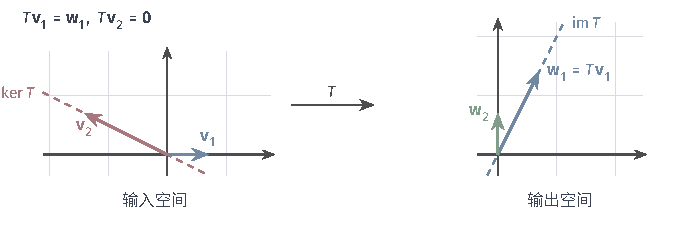
\includegraphics[width=112mm]{figures/00-shared/mathematical-preliminaries-upper/02-linear-spaces/tikz/comprehension-additions/equivalence-two-bases.pdf}
  \caption{两端独立选基化为秩标准形。$T(\bm x)=\bm A\bm x$，$\bm A=\left[\begin{smallmatrix}1&2\\2&4\end{smallmatrix}\right]$。左：输入基$\bm v_1=\bm e_1$（蓝）与$\bm v_2=(-2,1)^{\top}$（红），$\bm v_2$在核（红虚线）上。右：输出基$\bm w_1=T\bm v_1=(1,2)^{\top}$（蓝）位于像（蓝虚线）上，$\bm w_2=\bm e_2$（绿）补足一组基。在这两组基下$T$的矩阵为$\operatorname{diag}(1,0)$。}
  \label{fig:ls-equivalence-two-sided-bases-flow}
\end{figure}

\begin{theorem}[相抵判据]
\label{thm:ls-equivalence-criterion}
两个同形实矩阵$\bm A,\bm B\in\mathbb R^{m\times d}$相抵，当且仅当$\operatorname{rank}\bm A=\operatorname{rank}\bm B$。
\end{theorem}
\begin{proof}
必要性由式\eqref{eq:ls-equivalence-invariants}得到。充分性：设二者秩都为$r$，由上面的构造，存在可逆矩阵使$\bm R=\bm Q_A^{-1}\bm A\bm P_A=\bm Q_B^{-1}\bm B\bm P_B$，其中$\bm R$是式\eqref{eq:ls-rank-normal-form}的秩标准形。两式对接得$\bm B=(\bm Q_A\bm Q_B^{-1})^{-1}\bm A(\bm P_A\bm P_B^{-1})$，即二者相抵。
\end{proof}
所以固定形状以后，秩就是相抵的完整不变量：零矩阵只与零矩阵相抵，同形的满秩矩阵彼此相抵。把矩阵化到标准形的具体消元算法在第~\ref{chap:linear-equations-and-optimization}章建立。

\subsubsection{线性算子的换基与相似}
\label{sec:ls-similarity}
\phantomsection
\label{sec:ls-matrix-equivalences}

线性算子$T:V\to V$的输入与输出是同一个空间，记录时两端用同一组基；换基时，两端必须换成同一组新基。上面的推导加上这个约束会给出什么关系？同一个算子的两个方阵记录什么时候可以互相转化？

\paragraph{换基过程}
设$\mathcal B$与$\mathcal B'$是$V$的两组基，$\bm A=[T]_{\mathcal B}$、$\bm B=[T]_{\mathcal B'}$，记$\bm P=\bm S_{\mathcal B\leftarrow\mathcal B'}$，它的第$j$列是新基向量$\bm b'_j$在旧基$\mathcal B$下的坐标，$\bm P$可逆，反向换基矩阵为$\bm P^{-1}$。输入端与输出端是同一个空间、同一次换基，所以三步推导中的$\bm Q$也是$\bm P$：先把新坐标换成旧坐标，$[\bm v]_{\mathcal B}=\bm P[\bm v]_{\mathcal B'}$；在旧基下作用，$[T\bm v]_{\mathcal B}=\bm A\bm P[\bm v]_{\mathcal B'}$；再把输出换回新坐标，
\[
 [T\bm v]_{\mathcal B'}=\bm P^{-1}[T\bm v]_{\mathcal B}=\bm P^{-1}\bm A\bm P[\bm v]_{\mathcal B'}.
\]
与$[T\bm v]_{\mathcal B'}=\bm B[\bm v]_{\mathcal B'}$逐列比较，得到
\begin{equation}
 \bm B=\bm P^{-1}\bm A\bm P.
 \label{eq:linear-algebra-similarity-change-basis}
\end{equation}
这就是式~\eqref{eq:ls-equivalence-transform}取$\bm Q=\bm P$的情形。

\paragraph{相似的定义}
\phantomsection
\label{sec:ls-similarity-meaning}
与相抵一样，把同一算子两个记录之间的关系单独命名。
\begin{definition}[矩阵相似]
\label{def:ls-matrix-similarity}
设$\bm A,\bm B$是$n$阶方阵。若存在$n$阶可逆矩阵$\bm P$使$\bm B=\bm P^{-1}\bm A\bm P$，就称$\bm A$与$\bm B$\term{相似}（similar）。
\end{definition}
相似的两个矩阵正是同一个线性算子在两组基下的记录。一个方向由上面的推导给出；另一方向，给定$\bm A=[T]_{\mathcal B}$和可逆$\bm P$，以$\bm P$的各列为旧基坐标得到一组新基，$T$在其下的矩阵恰为$\bm P^{-1}\bm A\bm P$。

相似不要求$\bm A,\bm B$本身可逆，可逆的只是换基矩阵$\bm P$。取$\bm Q=\bm P$可见，相似的矩阵必定相抵；反之不然，下面的判定会给出秩相同、因而相抵却不相似的例子。

看一个具体例子：适当换基，可以把一个算子的矩阵化成对角形。
\begin{example}[换基把算子的矩阵化为对角形]
\label{ex:ls-similarity-diagonal}
给定：示例~\ref{ex:ls-plane-operator-matrix}中的算子$T(x_1,x_2)=(2x_1+x_2,3x_2)$，它在标准基下的矩阵为$\bm A=\left[\begin{smallmatrix}2&1\\0&3\end{smallmatrix}\right]$，即$T\bm e_1=2\bm e_1$、$T\bm e_2=\bm e_1+3\bm e_2$；新基取$\bm b_1'=\bm e_1$、$\bm b_2'=\bm e_1+\bm e_2$。

计算：$\bm P=\left[\begin{smallmatrix}1&1\\0&1\end{smallmatrix}\right]$，$\bm P^{-1}=\left[\begin{smallmatrix}1&-1\\0&1\end{smallmatrix}\right]$，
\[
 \bm B=\bm P^{-1}\bm A\bm P
 =\begin{bmatrix}1&-1\\0&1\end{bmatrix}
 \begin{bmatrix}2&1\\0&3\end{bmatrix}
 \begin{bmatrix}1&1\\0&1\end{bmatrix}
 =\begin{bmatrix}2&0\\0&3\end{bmatrix}.
\]
直接验证也是如此：$T\bm b_1'=2\bm b_1'$，$T\bm b_2'=T\bm e_1+T\bm e_2=3\bm e_1+3\bm e_2=3\bm b_2'$。

结论：在新基下，$T$的矩阵是对角矩阵$\operatorname{diag}(2,3)$；两个新基方向在$T$的作用下都只被伸缩、不被转向，彼此互不干扰。
\end{example}
$T$本身没有改变，改变的只是沿哪两条方向读取。图~\ref{fig:ls-similarity-change-of-basis-flow}把这一点画在平面上：在标准基下，单位正方形被$T$拉成一个斜的平行四边形，矩阵$\bm A$有非零的非对角元；在新基下，基向量围成的平行四边形只沿两条基方向分别伸长$2$倍和$3$倍，矩阵就是对角的$\bm B$。只被伸缩的方向称为特征方向；怎样系统地找到它们，什么时候能找到足够多的这种方向组成一组基，是第~\ref{chap:linear-analysis}章的问题。
\begin{figure}[!htb]
  \centering
  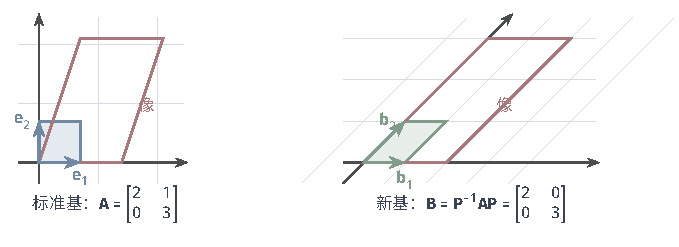
\includegraphics[width=112mm]{figures/00-shared/mathematical-preliminaries-upper/02-linear-spaces/tikz/comprehension-additions/similarity-two-bases.pdf}
  \caption{同一个算子在两组基下的记录。左：标准基$\bm e_1,\bm e_2$围成的单位正方形（蓝）被$\bm A=\left[\begin{smallmatrix}2&1\\0&3\end{smallmatrix}\right]$送到红色平行四边形，形状被斜切。右：新基$\bm b_1=\bm e_1$、$\bm b_2=\bm e_1+\bm e_2$围成的平行四边形（绿）被同一个算子送到红色平行四边形，只沿$\bm b_1$伸长$2$倍、沿$\bm b_2$伸长$3$倍，因此新矩阵为$\operatorname{diag}(2,3)$。浅色斜线为新基网格。}
  \label{fig:ls-similarity-change-of-basis-flow}
\end{figure}

\paragraph{相似不变量}
\phantomsection
\label{sec:ls-similarity-properties}
同一个算子的性质不应随基改变；哪些量在相似下保持不变？相似首先是等价关系：$\bm A=\bm I^{-1}\bm A\bm I$给出自反性；由$\bm B=\bm P^{-1}\bm A\bm P$得$\bm A=\bm P\bm B\bm P^{-1}$，给出对称性；若再有$\bm C=\bm Q^{-1}\bm B\bm Q$，则$\bm C=(\bm P\bm Q)^{-1}\bm A(\bm P\bm Q)$，给出传递性。这三条分别对应不换基、换回原基和连续换两次基。

相似是相抵的特例，相抵不变量自然保持：$\operatorname{null}(\bm B)=\bm P^{-1}\operatorname{null}(\bm A)$，$\operatorname{range}(\bm B)=\bm P^{-1}\operatorname{range}(\bm A)$，因此
\begin{equation}
\begin{gathered}
\operatorname{rank}\bm B=\operatorname{rank}\bm A\\
\dim\operatorname{null}(\bm B)=\dim\operatorname{null}(\bm A).
\end{gathered}
\label{eq:ls-similarity-invariants}
\end{equation}
算子还能反复作用，而先后作用与换基相容：若$\bm B_1=\bm P^{-1}\bm A_1\bm P$、$\bm B_2=\bm P^{-1}\bm A_2\bm P$，则
\begin{equation}
 \bm B_1\bm B_2
 =\bm P^{-1}\bm A_1\bm P\,\bm P^{-1}\bm A_2\bm P
 =\bm P^{-1}\bm A_1\bm A_2\bm P,
 \label{eq:ls-similarity-product}
\end{equation}
中间的$\bm P\bm P^{-1}$相消。归纳得$\bm B^k=\bm P^{-1}\bm A^k\bm P$：反复作用同一个算子，在新基下仍是同一过程的记录。同样，对任意实数$c$，$\bm B-c\bm I=\bm P^{-1}(\bm A-c\bm I)\bm P$，所以$\bm A-c\bm I$与$\bm B-c\bm I$也相似，由式~\eqref{eq:ls-similarity-invariants}，
\begin{equation}
\begin{gathered}
\operatorname{rank}(\bm B-c\bm I)=\operatorname{rank}(\bm A-c\bm I)\\
c\in\mathbb R.
\end{gathered}
\label{eq:ls-similarity-shifted-rank}
\end{equation}
这比总秩更细：它对每个$c$都给出一个不变量。

相似还保持两个可以直接计算的标量。由行列式的乘法性（第~\ref{sec:ls-determinant-properties}节）与$\det(\bm P^{-1})\det\bm P=\det\bm I=1$，
\[
 \det(\bm P^{-1}\bm A\bm P)=\det(\bm P^{-1})\,\det\bm A\,\det\bm P=\det\bm A;
\]
由迹的循环性（式~\eqref{eq:linear-algebra-trace-cyclic}），
\[
 \operatorname{tr}(\bm P^{-1}\bm A\bm P)=\operatorname{tr}\bigl((\bm A\bm P)\bm P^{-1}\bigr)=\operatorname{tr}\bm A.
\]
两式说明，行列式与迹只依赖算子本身，是判断两个矩阵能否记录同一算子时可以直接计算的两个标量不变量。例如示例~\ref{ex:ls-similarity-diagonal}中的$\bm A$与$\bm B=\operatorname{diag}(2,3)$行列式都是$6$，迹都是$5$。于是可以说“算子$T$的行列式”“算子$T$的迹”，用任意一组基下的矩阵计算即可。

引入特征值以后还将看到（第~\ref{sec:ls-eigen-similarity-invariance}节），特征值与特征多项式同样是相似不变量，而行列式与迹恰好是特征值之积与特征值之和。一般的换基不保持欧氏长度与夹角，这些度量量不在相似保持之列。

\paragraph{相似的判定}
\phantomsection
\label{sec:ls-similarity-conditions}
怎样判断两个给定的方阵是否相似？两端左乘$\bm P$，相似等价于存在\emph{可逆}的$\bm P$满足
\begin{equation}
 \bm A\bm P=\bm P\bm B.
 \label{eq:ls-similarity-equation}
\end{equation}
这是关于$\bm P$各元素的一组线性方程。只找到非零但不可逆的解还不够：那只是两个坐标子空间之间的对应，不是两组基之间的换基。

不变量给出否定的判据：只要某个相似不变量不同，两个矩阵就不相似。但秩、行列式、迹相同，都只是相似的必要条件，下面的例子说明它们合在一起也不够。
\begin{example}[反例：相抵而不相似的两个矩阵]
\label{ex:ls-equivalent-not-similar}
给定：$\bm I_2$与$\bm J=\left[\begin{smallmatrix}1&1\\0&1\end{smallmatrix}\right]$。

验证：二者都可逆，秩都为$2$，由相抵判据它们相抵；二者的行列式都是$1$，迹都是$2$。但取$c=1$，$\bm I_2-\bm I_2=\bm0$的秩为$0$，而$\bm J-\bm I_2=\left[\begin{smallmatrix}0&1\\0&0\end{smallmatrix}\right]$的秩为$1$，式~\eqref{eq:ls-similarity-shifted-rank}不成立。更直接地，若$\bm J=\bm P^{-1}\bm I_2\bm P$，则$\bm J=\bm P^{-1}\bm P=\bm I_2$，矛盾。

结论：$\bm I_2$与$\bm J$相抵，秩、行列式与迹也都相同，却不相似；单位矩阵只与自己相似。
\end{example}
这正是“两端换基相同”这一约束的代价：相抵时秩相同就足够，相似时连秩、行列式与迹一起相同都不够。比较$\bm A-c\bm I$在各个$c$处的秩是更细的必要条件；完整的相似分类需要Jordan标准形，本书不展开。

\subsection{多线性映射}

此前的线性映射只有一个输入。矩阵的元素内积、两个向量的外积却各有两个输入：固定其中一个，再改变另一个时，结果保持线性组合。为了表达这种逐个输入的线性，可以为每个输入保留一个独立的槽位。

设$V_1,\ldots,V_k,W$是同一数域上的线性空间。映射$F:V_1\times\cdots\times V_k\to W$若在固定其余输入后，对每一个输入分别都是线性的，就称为多线性映射；$k=2$时称为双线性映射。例如$F(\bm x,\bm y)=\bm x\bm y^\top$对两个输入分别线性。

分别线性不等于把输入对看成一个整体以后仍线性：对实数乘法$f(x,y)=xy$，有$f(1,1)+f(1,1)=2$，但$f(2,2)=4$。

各输入空间和输出空间选定基后，多线性映射也能由有限组系数记录。以实双线性标量映射$B:V\times W\to\mathbb R$为例，取基$(\bm v_i)$与$(\bm w_j)$，令$b_{i,j}=B(\bm v_i,\bm w_j)$。当$\bm x=\sum_i x_i\bm v_i$、$\bm y=\sum_j y_j\bm w_j$时，逐个槽位展开得到
\[
 B(\bm x,\bm y)=\sum_{i,j}x_i y_j b_{i,j}.
\]
因此，基向量两两配对的结果足以恢复任意输入的值。换基改变这些系数，映射本身不变；它与上一章数组的张量积和指标收缩有关，但不能把改变数组存放次序直接等同于改变坐标基。

% 第5章第4节：对偶空间（线性泛函与对偶空间、对偶基、对偶映射与转置）。

\section{对偶空间}
\label{sec:ls-dual-spaces}

线性映射把对象送到另一个空间；还有一类最简单的作用，只把对象读成一个数。取多项式在某一点的值、取信号的第一个样本、计算一组特征的加权和，都是这样的读取；第~\ref{sec:ls-coordinates}节的坐标$x_j$也是，每个坐标都把对象读成一个数。第~\ref{chap:linear-operations}章在$\mathbb R^d$上用内积$\langle\bm w,\bm x\rangle$表示加权读取，读取规则借一个向量$\bm w$来写；一般空间上还没有内积，读取规则本身是什么对象，就需要单独回答。

本节讨论三个问题：全部线性读取组成怎样的空间；坐标作为读取，与基有怎样的关系；对象经过线性映射以后，输出端的读取怎样传回输入端。最后一个问题的答案是转置，它给第~\ref{chap:linear-operations}章中“行列互换”的操作一个不依赖坐标的含义。回答这三个问题只用到线性运算；读取规则的大小需要范数，留到下一章讨论。

\subsection{线性泛函与对偶基}
\label{sec:ls-dual-space}

\paragraph{线性泛函}
保持线性组合的标量读取称为\term{线性泛函}（linear functional）：映射$\varphi:V\to\mathbb R$满足
\[
\begin{gathered}
\varphi(a\bm x+b\bm y)=a\varphi(\bm x)+b\varphi(\bm y)\\
\bm x,\bm y\in V,\ a,b\in\mathbb R.
\end{gathered}
\]
它就是陪域为$\mathbb R$的线性映射。在$P_k$上，取值$p\mapsto p(t_0)$与积分$p\mapsto\int_0^1p(t)\,\mathrm dt$都是线性泛函；在$\mathbb R^d$上，读取第$j$个坐标与加权和$\bm x\mapsto\bm a^\top\bm x$都是线性泛函。但并非每个把向量读成一个数的规则都是线性泛函。
\begin{example}[反例：两个非线性的读取]
\label{ex:ls-nonlinear-readouts}
给定：$\mathbb R^d$上的两个读取$\varphi_1(\bm x)=x_1+1$与$\varphi_2(\bm x)=\lVert\bm x\rVert_2$。

验证：线性泛函必把零向量读成$0$，而$\varphi_1(\bm0)=1$。线性泛函还满足$\varphi(-\bm x)=-\varphi(\bm x)$；但对任一$\bm x\neq\bm0$，$\varphi_2(-\bm x)=\lVert\bm x\rVert_2>0$，而$-\varphi_2(\bm x)<0$。

结论：$\varphi_1$与$\varphi_2$都不是线性泛函。
\end{example}

按线性映射的矩阵表示，选定$V$的基$\mathcal B=(\bm b_1,\ldots,\bm b_d)$、输出端取数$1$作基，线性泛函$\varphi$记录为$1\times d$矩阵
\[
 \begin{gathered}
[\varphi]_{\mathcal B}=\bigl(\varphi(\bm b_1),\ \ldots,\ \varphi(\bm b_d)\bigr)\\
\varphi(\bm v)=[\varphi]_{\mathcal B}[\bm v]_{\mathcal B}=\sum_{j=1}^dx_j\varphi(\bm b_j).
 \end{gathered}
\]
对象的坐标是一列，读取规则的系数是一行，二者相乘得到读数。

非零泛函取到某个非零值，把相应的输入缩放即可取到任意实数，所以它的像是整个$\mathbb R$；由秩零度定理，它的核是$d-1$维子空间。读数等于$c$的点组成核的平移$\bm x_0+\ker\varphi$（其中$\varphi(\bm x_0)=c$），在平面上就是一族平行直线。

\paragraph{对偶空间}
同一个对象可以接受多种读取，两种读取也可以组合：规定
\[
 (\alpha\varphi+\beta\psi)(\bm x)=\alpha\varphi(\bm x)+\beta\psi(\bm x),
\]
右端对$\bm x$仍保持线性组合，所以线性泛函的线性组合仍是线性泛函。全部线性泛函在这两种运算下构成线性空间，称为$V$的\term{对偶空间}（dual space），记为$V^*$。输入向量是被读取的对象，泛函是读取规则，二者属于不同的空间；即使在$\mathbb R^d$中一行系数与一列坐标的数字相同，也不能直接相加。

\paragraph{对偶基}
$V^*$有多大？坐标给出了一组现成的读取。对$V$的有序基$\mathcal B=(\bm b_1,\ldots,\bm b_d)$，第$j$个坐标$\bm v\mapsto x_j$是线性泛函（坐标映射保持线性组合），记为$\varphi_j$。由$\bm b_i$的坐标是$\bm e_i$，
\begin{equation}
 \varphi_j(\bm b_i)=\delta_{j,i}
 =\begin{cases}1,&i=j,\\0,&i\neq j.\end{cases}
 \label{eq:ls-dual-basis-def}
\end{equation}
反过来，线性泛函由它在基向量上的值决定，所以式~\eqref{eq:ls-dual-basis-def}也可以当作$\varphi_j$的定义。

这$d$个读取构成$V^*$的一组基。任意$\varphi\in V^*$都能写成
\[
 \varphi=\sum_{j=1}^d\varphi(\bm b_j)\,\varphi_j,
\]
因为两边在每个$\bm b_i$上取值都是$\varphi(\bm b_i)$，而线性泛函由基向量上的值决定。

若$\sum_ja_j\varphi_j=0$，在$\bm b_i$上取值得$a_i=0$，所以它们线性无关。这组$\varphi_1,\ldots,\varphi_d$称为$\mathcal B$的\term{对偶基}（dual basis），于是$\dim V^*=\dim V$。读取$\varphi$在对偶基下的坐标正是它在各基向量上的读数$\varphi(\bm b_j)$，即上面那一行系数。

对偶基的每个成员依赖整组基，而不只依赖对应的那个基向量。
\begin{example}[改变第二个基向量会改变第一个坐标读取]
\label{ex:ls-dual-basis-depends-on-basis}
给定：$\mathbb R^2$的标准基$(\bm e_1,\bm e_2)$与基$(\bm e_1,\bm e_1+\bm e_2)$。

计算：标准基的对偶基是两个坐标读取$\varphi_1(x,y)=x$、$\varphi_2(x,y)=y$。在第二组基下，
\[
 (x,y)^\top=(x-y)\bm e_1+y(\bm e_1+\bm e_2),
\]
所以第一个坐标读取变成$x-y$，第二个坐标读取仍是$y$。

结论：两组基的第一个向量都是$\bm e_1$，相应的第一个对偶读取却从$x$变成了$x-y$。
\end{example}
对一般的基，对偶基要由方程组$\varphi_j(\bm b_i)=\delta_{j,i}$解出。
\begin{example}[斜基的对偶基]
\label{ex:ls-dual-basis-oblique}
给定：$\mathbb R^2$的基$\bm b_1=(2,1)^\top$、$\bm b_2=(-1,1)^\top$，以及读取横坐标的泛函$\ell(x,y)=x$。

计算：设$\varphi_1(x,y)=\alpha x+\beta y$。条件$\varphi_1(\bm b_1)=2\alpha+\beta=1$与$\varphi_1(\bm b_2)=-\alpha+\beta=0$给出$\alpha=\beta=1/3$；同样由$\varphi_2(\bm b_1)=0$、$\varphi_2(\bm b_2)=1$解出$\varphi_2$，得
\[
 \begin{gathered}
\varphi_1(x,y)=\frac{x+y}3\\
\varphi_2(x,y)=\frac{-x+2y}3 .
 \end{gathered}
\]
$\ell$在基向量上的读数为$\ell(\bm b_1)=2$、$\ell(\bm b_2)=-1$，所以$\ell=2\varphi_1-\varphi_2$。代入验证：$\tfrac23(x+y)-\tfrac13(-x+2y)=x$。

结论：$\ell$在对偶基下的坐标是$(2,-1)$，正是它在两个基向量上的读数。
\end{example}
图~\ref{fig:ls-dual-basis-readout}画出这些读取：每个对偶读取只在一个基向量上读到$1$，在另一个基向量上读到$0$。
\begin{figure}[htbp]
  \centering
  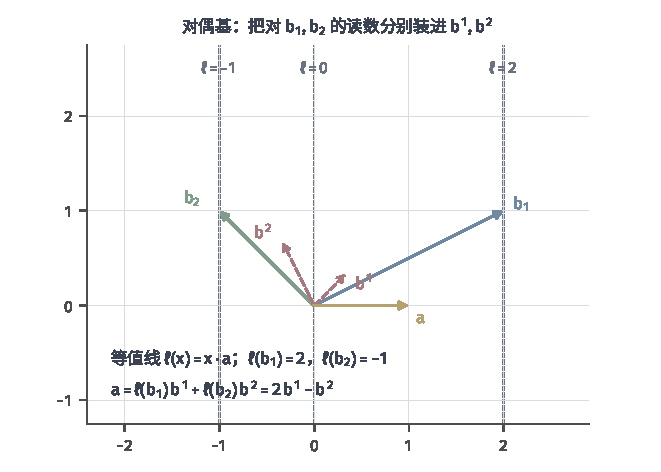
\includegraphics[width=112mm]{figures/00-shared/mathematical-preliminaries-upper/02-linear-spaces/matplotlib/ls-dual-basis-readout/ls-dual-basis-readout.pdf}
  \caption{对偶读取的几何示意。蓝箭头$\bm b_1=(2,1)$、绿箭头$\bm b_2=(-1,1)$为基向量；红色虚线箭头$\bm b^1=(1/3,1/3)$、$\bm b^2=(-1/3,2/3)$分别是对偶基$\varphi_1,\varphi_2$的系数向量，即$\varphi_i(\bm x)=\bm b^i\cdot\bm x$，满足$\varphi_i(\bm b_j)=\delta_{i,j}$。把读取规则画成平面箭头借用了标准内积，这一对应在第~\ref{sec:ls-riesz-representation}节说明。黄色箭头$\bm a=(1,0)$给出读取$\ell(\bm x)=\bm a\cdot\bm x$，灰色虚线为等值线$\ell=c$（$c=-1,0,2$）；$\ell(\bm b_1)=2$、$\ell(\bm b_2)=-1$，且$\bm a=2\bm b^1-\bm b^2$。}
  \label{fig:ls-dual-basis-readout}
\end{figure}

换基时，读取系数与坐标的变化方向相反。

设新基$\mathcal B'$由换基矩阵$\bm P=\bm S_{\mathcal B\leftarrow\mathcal B'}$给出，即$\bm b'_j=\sum_i\bm P_{i,j}\bm b_i$。坐标按$[\bm v]_{\mathcal B'}=\bm P^{-1}[\bm v]_{\mathcal B}$变化；读取系数则按$\varphi(\bm b'_j)=\sum_i\varphi(\bm b_i)\bm P_{i,j}$变化，即$[\varphi]_{\mathcal B'}=[\varphi]_{\mathcal B}\bm P$。二者相乘时$\bm P$与$\bm P^{-1}$相消，读数$\varphi(\bm v)$不随基改变，这正是读数应有的性质。

\subsection{对偶映射}
\label{sec:ls-dual-map}

已知线性映射$T:V\to W$和输出端的一个读取$f\in W^*$，输入$\bm x$经过$T$以后被读成$f(T\bm x)$。先作用、再读取，合起来是输入端的一个读取。由这一复合定义\term{对偶映射}（dual map）$T':W^*\to V^*$：
\begin{equation}
\begin{gathered}
T'f=f\circ T\\
(T'f)(\bm x)=f(T\bm x).
\end{gathered}
\label{eq:ls-dual-map-def}
\end{equation}
$T'$保持线性组合：$(T'(\alpha f+\beta g))(\bm x)=\alpha f(T\bm x)+\beta g(T\bm x)$。对象从$V$走到$W$，读取则从$W^*$传回$V^*$，方向相反；这只是把读取规则搬回输入端，并不是对$T$求逆。复合时次序也随之反转：对$S:W\to U$，$(S\circ T)'f=f\circ S\circ T=T'(S'f)$，即$(S\circ T)'=T'\circ S'$。

\paragraph{对偶映射的矩阵是转置}
设输入基$\mathcal B=(\bm b_1,\ldots,\bm b_d)$、输出基$\mathcal C=(\bm c_1,\ldots,\bm c_m)$下$T$的矩阵为$\bm A$，即$T\bm b_j=\sum_ka_{k,j}\bm c_k$；两组基的对偶基分别记为$\varphi_1,\ldots,\varphi_d$与$\psi_1,\ldots,\psi_m$。取输出读取$f=\sum_iy_i\psi_i$，它传回输入端以后，在输入基向量上的读数是
\[
 (T'f)(\bm b_j)=f(T\bm b_j)
 =\sum_iy_i\,\psi_i\Bigl(\sum_ka_{k,j}\bm c_k\Bigr)
 =\sum_ia_{i,j}y_i=(\bm A^\top\bm y)_j .
\]
上一小节说明，读取在对偶基下的坐标就是它在各基向量上的读数，所以$T'f$的坐标为$\bm A^\top\bm y$：在对偶基下，对偶映射的矩阵是$\bm A^\top$。转置的乘积规则$(\bm B\bm A)^\top=\bm A^\top\bm B^\top$正是$(S\circ T)'=T'\circ S'$的坐标记录。下面用一个具体映射核对这一结论。
\begin{example}[把输出的第一个分量读取传回输入端]
\label{ex:ls-dual-map-first-component}
给定：$T(x_1,x_2)=(2x_1+x_2,\ 3x_2)$，它在标准基下的矩阵为$\bm A=\left[\begin{smallmatrix}2&1\\0&3\end{smallmatrix}\right]$；输出端读取第一个分量，即$f=\psi_1$，系数$\bm y=(1,0)^\top$。

计算：先作用再读取，$(T'f)(\bm x)=f(T\bm x)=2x_1+x_2$，系数为$(2,1)^\top$。按矩阵计算，$\bm A^\top(1,0)^\top=(2,1)^\top$。

结论：两种算法一致，传回的读取系数正是$\bm A$的第一行。
\end{example}
一般地，读取输出第$i$个分量并传回输入端，得到的读取系数就是$\bm A$的第$i$行，所以$T'$的像在坐标下就是行空间。

\paragraph{再证行秩等于列秩}
对偶映射给出定理~\ref{thm:ls-row-rank-column-rank}的一个不依赖消元的证明。先看$T'$的核。$T'f=0$意味着$f(T\bm x)=0$对一切$\bm x$成立，即$f$在$\operatorname{im}T$上恒为零：$\ker T'$由看不见任何可达输出的读取组成，在坐标下就是$\bm A^\top\bm y=\bm0$，即左零空间。

再算它的维数。

设$r=\operatorname{rank}T$，取$\operatorname{im}T$的基$\bm c_1,\ldots,\bm c_r$并扩充为$W$的基$\bm c_1,\ldots,\bm c_m$，对偶基为$\psi_1,\ldots,\psi_m$。读取$f=\sum_iy_i\psi_i$在$\operatorname{im}T$上恒为零，当且仅当它在$\bm c_1,\ldots,\bm c_r$上都读到零，即$y_1=\cdots=y_r=0$，所以$\ker T'=\operatorname{span}\{\psi_{r+1},\ldots,\psi_m\}$，维数为$m-r$。

对$T':W^*\to V^*$用秩零度定理，$\operatorname{rank}T'=\dim W^*-\dim\ker T'=m-(m-r)=r$。$T'$的矩阵是$\bm A^\top$，于是$\operatorname{rank}\bm A^\top=\operatorname{rank}\bm A$。

至此，读取规则有了自己的空间、坐标和传递规律。还有两个问题没有回答。一个读取有多“大”，即输入有界时读数最多有多大？要回答这个问题，需先规定输入的范数；下一章将定义对偶范数（第~\ref{sec:ls-dual-norms}节）。一个读取能否写成与某个固定向量的配对？这要用到内积，在第~\ref{sec:ls-riesz-representation}节回答。

\section{本章小结}
\label{sec:ls-representation-summary}

线性空间规定哪些对象可以相加、缩放，子空间保留这些运算，直和描述唯一分解，而商空间把子空间内的差别视为相同。基同时满足张成与线性无关，因此每个向量都有唯一坐标；换基改变坐标，却不改变向量本身。

线性映射保持线性组合，其核与像分别记录丢失的输入和能够到达的输出。选定两端的基后，映射由矩阵表示；两端独立换基得到相抵，同一空间两端使用同一组基则得到相似。对偶空间由线性泛函组成，对偶映射把输出端的读取传回输入端，在对偶基下记录为转置。

这些结构尚未规定向量的大小或方向之间的夹角。下一章引入范数和内积，讨论收敛、正交分解与最佳近似，再为谱和方程的研究准备工具。

